\documentclass{fast_latex}
% yay! We can use any kind of funky diacritic:
\usepackage[utf8]{inputenc}

\usepackage{lastpage}
\usepackage{setspace}
\usepackage{graphicx}
\usepackage[pdfborder={0 0 0}]{hyperref}		% turn on when latex is used (not miktec)
\usepackage{url} % LEO: urls \url{}
\usepackage{verbatim} % code and comment
\usepackage{longtable}
\usepackage{xspace}   % whitespace after a macro if no punctuation after the macro
\usepackage{multirow}
\usepackage{colortbl}
\usepackage{longtable}
\usepackage{array}
\usepackage{amssymb}
\usepackage{paralist}

% This is useful for switching in-line comments on and off!
\usepackage{ifthen}
\newboolean{showcomments}
\setboolean{showcomments}{true}
\ifthenelse{\boolean{showcomments}}
{
	\definecolor{Red}{rgb}{1,0,0}
	\newcommand{\note}[1]{\begin{scriptsize}{{\textsf{\textbf{{\textcolor{Red}{[[#1]]}}}}}}\end{scriptsize}}
	\definecolor{Orange}{rgb}{1,0.5,0}
	\newcommand{\todo}[1]{\textsf{\textbf{\textcolor{Orange}{[[TODO: #1]]}}}}
    \definecolor{Green}{rgb}{0,1,0}
    \newcommand{\commentreply}[1]{\begin{scriptsize}{\textsf{\textbf{\textcolor{Green}{[[#1]]}}}}\end{scriptsize}}
} {
	\newcommand{\note}[1]{\textbf{}}
	\newcommand{\todo}[1]{}
    \newcommand{\commentreply}[1]{}
}


\usepackage{listings}

\lstdefinelanguage{turtle} 
{morekeywords={@prefix, a}, 
sensitive=false, 
morecomment=[l]{\#}, 
morestring=[b]",
}

\lstdefinelanguage{sparql} 
{morekeywords={PREFIX, a, SELECT, CONSTRUCT, WHERE, UNION, OPTIONAL, FILTER, DISTINCT, ORDER, BY, GRAPH}, 
sensitive=false, 
morecomment=[l]{\#}, 
morestring=[b]",
}

\lstset{
	captionpos=b, 
	extendedchars=true,
	basicstyle=\footnotesize \sffamily, 
	stringstyle=\bfseries,
	frame=single,
	frameround=tttt,
	showstringspaces=false,
	breaklines=true,
	% inputencoding=utf8,
}


\parindent0pt

\newcommand\deliverableNumber{D2.2.2}
\newcommand\deliverableTitle{Ontology and Conceptual Model for the Semantic Characterisation of Complex Gadgets}
\newcommand\deliverableTitleShort{Ontology and Conceptual Model}
\newcommand\workpackageNumber{2}
\newcommand\workpackageTitle{Definition of Conceptual Model}
\newcommand\authorOne{Knud M\"oller, NUIG}
\newcommand\authorTwo{Ismael Rivera, NUIG}
\newcommand\authorThree{Author 3}
\newcommand\authorFour{Author 4}
\newtheorem{example}{\emph{Example}}

\begin{document}
% explicit hyphenations
\hyphenation{RDF-Re-po-si-to-ry}
\hyphenation{name-space}
\hyphenation{So-cket-A-dap-ter}

%\fontfamily{tahoma}\selectfont
\def\note#1{\marginpar{\footnotesize#1}} % use this to show the notes in the document
%\def\note#1{} % use this to hide the notes



%%%%%%%%%%%%%%%%%%%%%%%%%%%%%%%%%%%%%%%%%%%%%%%%%%%%%%%%%%%%%%%%%%%%%%%%%%%%%%%%
% TITLE PAGES 
%%%%%%%%%%%%%%%%%%%%%%%%%%%%%%%%%%%%%%%%%%%%%%%%%%%%%%%%%%%%%%%%%%%%%%%%%%%%%%%%
\thispagestyle{empty}

\pagenumbering{roman}

\begin{flushright}
	
\includegraphics[width=3cm]{images/FP7_logo}
\end{flushright}

\vspace{1cm}

%\begin{minipage}[p]{15cm}
	\begin{center}
		
\includegraphics{images/FAST_logo}\\
		\vspace{1cm}
		{\LARGE{\sffamily \emph{FAST AND ADVANCED STORYBOARD TOOLS}}}\\
		\vspace{0.5cm}
		{\LARGE \sffamily \emph{FP7-ICT-2007-1-216048}}\\
		\vspace{0.5cm}
		{\LARGE \sffamily \emph{http://fast.morfeo-project.eu}}\\
		\vspace{4cm}
		{\LARGE \sffamily \textbf{Deliverable \deliverableNumber}}\\
		\vspace{0.5cm}
		{\LARGE \sffamily \textbf{\deliverableTitle}}\\
		\vspace{2cm}
		{\large \sffamily \authorOne}\\
		{\large \sffamily \authorTwo}\\
		\vspace{0.5cm}
		\vfill
		{\large \sffamily Date: 27/02/2010}\\
		\vspace{1cm}
		{\sffamily FAST is partially funded by the E.C. (grant code: FP7-ICT-2007-1-216048).}
		
	\end{center}
%\end{minipage}


\clearpage
%%%%%%%%%%%%%%
% NEXT PAGES %
%%%%%%%%%%%%%%
\pagestyle{scrheadings}

\lohead{
\includegraphics[width=4cm]{images/FAST_logo_transparent}}
%\cohead{\small\textcolor{fast@lightgrey}{\deliverableTitle}}
%\rohead{\small{\today}}
%\lofoot{\small\textcolor{fast@lightgrey}{Task Force Ontologies}}
\cofoot{\small{FAST 216048 --- \deliverableTitleShort}}
\rofoot{\small{\thepage}}

\newpage
%
%\section*{Authors}
%\authorOne \\
%%\authorTwo \\
%%\authorThree\\
%%\authorFour\\
%
%
%\vfill
%%\section*{Project Co-ordinator}
%%\hspace*{-2,5cm}\begin{minipage}[p]{14cm}
%%Dr. Ansgar Bernardi \\
%%German Research Center for Artificial Intelligence (DFKI) GmbH \\
%%Trippstadter Strasse 122 \\
%%D 67663 Kaiserslautern \\
%%Germany \\
%%Email: bernardi@dfki.uni-kl.de, phone: +49 631 205 3582, fax: +49 631 205 4910 \\
%%\end{minipage}
%
%
%\section*{Partners}
%Telef\'onica Investigaci\'on y Desarrollo (Telef\'onica I+D), Spain \\
%National University of Ireland, Galway (NUIG), Republic of Ireland \\
%Kassel University, Germany \\
%Cyntelix Corporation, Republic of Ireland \\
%SAP AG, Germany \\
%Universidad Polit\'ecnica de Madrid (UPM), Spain
%
%
%\vspace{0.3cm}
%\begin{footnotesize}
%Copyright: FAST Consortium 2009\\
%\end{footnotesize}

%\clearpage


\section*{Version History}

\begin{small}
\begin{tabular}{|l|l|l|p{7.5cm}|}
\hline
\rowcolor{fast@lightgrey}\textcolor{white}{\textbf{Rev. No.}} &
                            \textcolor{white}{\textbf{Date}} &
                            \textcolor{white}{\textbf{Author (Partner)}} &
							\textcolor{white}{\textbf{Change description}}\\ \hline
%0.1 & 15.12.2008 & Knud M\"oller (NUIG) & template modelled \\ \hline
%0.2 & 15.02.2009 & Knud M\"oller (NUIG) & content moved from wiki after internal review \\ \hline
1.0 & 27.02.2009 & Knud M\"oller (NUIG) & final version (D2.2.1) ready for external review \\ \hline
2.0 & 27.02.2010 & Knud M\"oller (NUIG) & final version (D2.2.2) ready for external review \\ \hline
\end{tabular}
\end{small}

\color{black}

\vfill
%{\bf Explanations of abbreviations on front page}\\
%\\
%%Nature \\
%R: Report \\
%P: Prototype \\
%R/P: Report and Prototype \\
%O: Other \\
% \\
%Dissemination level \\
%PU: Public \\
%PP: Restricted to other FP6 participants \\
%RE: Restricted to specified group \\
%CO: Confidential, only for NEPOMUK partners \\

\newpage

%%%%%%%%%%%%%%%%%%%%%
% Executive Summary %
%%%%%%%%%%%%%%%%%%%%%

\clearpage

\section*{Executive Summary}
\doublespacing

This deliverable defines the ontology and conceptual model for the semantic characterisation of complex gadgets in the FAST project. As such, it feeds directly into the various implementation efforts within the project. In the document, we present the ontology development methodology (Methontology) and design principles we have applied. Following Methontology, our design and development process results in a number of different living documents, which both function as a development tool, as well as documentation for the ontology itself. The major part of the deliverable is made up of these documents, resulting in the final \emph{implementation document} which formally defines the ontology in OWL DL semantics.

\newpage

%%%%%%%%%%%%%%%%%%%%%
% Document Summary %
%%%%%%%%%%%%%%%%%%%%%

\clearpage

\section*{Document Summary}
% double spacing from here on:
\singlespacing
\begin{small}

\begin{tabular}
	%{| >{\columncolor{fast@lightgrey}}p{3.25cm}|p{6cm}|p{2cm}|p{2cm}|}
	{| >{\columncolor{fast@lightgrey}}p{3.25cm}|p{6cm}|p{2cm}|p{2cm}|}
	\hline
	\textcolor{white}{\textbf{Code}} & {FP7-ICT-2007-1-216048} & {\textbf{Acronym}} & {FAST}\\ \hline
	\textcolor{white}{\textbf{Full title}} & \multicolumn{3}{l|}{Fast and Advanced Storyboard Tools}\\ \hline
	\textcolor{white}{\textbf{URL}} & \multicolumn{3}{l|}{\url{http://fast.morfeo-project.eu}}\\ \hline
	\textcolor{white}{\textbf{Project officer}} & \multicolumn{3}{l|}{Annalisa Bogliolo}\\ \hline
\end{tabular}

\vspace{0.5cm}

\begin{tabular}
	{| >{\columncolor{fast@lightgrey}}p{3.25cm}|p{1.25cm}|p{1cm}|p{1cm}|p{6.32cm}|}
	\hline
	\textcolor{white}{\textbf{Deliverable}} & {\textbf{Number}} & {\deliverableNumber} & {\textbf{Name}} & {\deliverableTitle}\\ \hline
	\textcolor{white}{\textbf{Work package}} & {\textbf{Number}} & {\workpackageNumber} & {\textbf{Name}} & {\workpackageTitle}\\ \hline
\end{tabular}

\vspace{0.5cm}

\begin{tabular}
	{| >{\columncolor{fast@lightgrey}}p{3.25cm}|p{1.4cm}|p{3.28cm}|p{1.6cm}|p{3.29cm}|}
	\hline
	\textcolor{white}{\textbf{Delivery data}} & {\textbf{Due date}} & {28/02/2010} & {\textbf{Submitted}} & {27/02/2010}\\ \hline
	\textcolor{white}{\textbf{Status}} & \multicolumn{2}{l|}{} & \multicolumn{2}{l|}{final}\\ \hline
	\textcolor{white}{\textbf{Dissemination Level}} & \multicolumn{4}{l|}{Public $\boxtimes$ / Consortium $\square$}\\ \hline
	\textcolor{white}{\textbf{Short description of contents}} & \multicolumn{4}{p{10.85cm}|}{\deliverableNumber{} is the second iteration of the FAST Gadget ontology. The ontology provides a formal description of the conceptual model of FAST in general, and of the screen/screenflow architecture in particular. The document comprises a discussion of the ontology development methodology used, a number of intermediate representations which document the development process, and the final product in the form of an OWL ontology.}\\ \hline
	\textcolor{white}{\textbf{Authors}} & \multicolumn{4}{l|}{\authorOne, \authorTwo}\\
%	{} & \multicolumn{4}{l|}{}\\ 
%	{} & \multicolumn{4}{l|}{}\\ 
%	{} & \multicolumn{4}{l|}{}\\
	\hline
	\textcolor{white}{\textbf{Deliverable Owner}} & \multicolumn{2}{l|}{\authorOne} & \textbf{email} & {knud.moeller@deri.org} \\ \cline{4-5}
	\textcolor{white}{\textbf{(Partner)}} & \multicolumn{2}{l|}{} & \textbf{phone} & {+353 91 495086} \\ \hline
	\textcolor{white}{\textbf{Keywords}} & \multicolumn{4}{p{10.85cm}|}{FAST, conceptual model, ontology, OWL, RDFS}\\ \hline
\end{tabular}
\end{small}
\newpage

%%%%%%%%%%%%%%%%%%%%%
% TABLE OF CONTENTS %
%%%%%%%%%%%%%%%%%%%%%
\doublespacing
\setcounter{tocdepth}{3}
\tableofcontents
\cleardoublepage
\pagenumbering{arabic}

%%%%%%%%%%%%%%%%%%%%%%%%%
% BEGINNING OF SECTIONS %
%%%%%%%%%%%%%%%%%%%%%%%%%
\clearpage
\rofoot{\small{Page \thepage\ of \pageref{LastPage}}}

\section{Introduction} % (fold)
\label{sec:introduction}

\subsection{Goal and Scope} % (fold)
\label{sub:goal_and_scope}

As the corner stone of the theoretical work undertaken in the FAST project, the definition of a conceptual model and ontology for the characterisation of complex gadgets feeds directly into the project's three main development activities: the development environment for complex gadgets (GVS), the development of gadget components and the semantic catalogue which represents the backend of the architecture. For all these different aspects of FAST, the ontology developed and presented in this deliverable provides a structured definition of their common domain of discourse. The ontology formally defines the parts which a complex gadget is made of, how the parts interrelate, what kind of metadata is available for each part, how users of the system are represented, etc.

While following an ontology design methodology which is agnostic to particular data models or implementation languages (see Appendix A), we have chosen to represent the final ontology specification using the Resource Description Framework (RDF) and OWL semantics.

In FAST, we have adopted the term \emph{gadget} for the small, Web-based software components which the project focusses on. There are small differences in meaning between this term and the term \emph{widget}, which is also widely used. However, for the purpose of this document, it should be noted that whenever we use the term \emph{gadget}, we also refer to what \emph{widget} at the same time.

% subsection goal_and_scope (end)

\subsection{Structure of the Document} % (fold)
\label{sub:structure_of_the_document}

This deliverable is structured as follows: as part of the introduction, we will present the methodology we chose to adopt for the development of the FAST gadget ontology, by discussing  each of its proposed stages in detail. Following, we will conclude the introduction by elaborating more on some of the general design decisions we are following. After briefly addressing the topic of related work in Sect.~\ref{sec:related_work} --- which is mainly covered in a different deliverable from this work package, \cite{urmetzer2010fast_state_of_the_art} --- the structure of the remainder of this document follows directly from our adopted methodology: we will perform a domain analysis in Sect.~\ref{sec:domain_analysis}, covering the stages of specification, conceptualisation and integration of existing vocabularies. This is then followed by the implementation step in Sect.~\ref{sec:ontology}, which covers the ontology in its final form (at this moment of the project). Finishing the deliverable, we present our conclusions and outlook on years two and three of the project in Sect.~\ref{sec:conclusions}.

% subsection structure_of_the_document (end)

\subsection{Changes from Previous Version} % (fold)
\label{sub:changes_from_previous_version}

The following changes have been made with respect to the previous version of this deliverable, D2.2.1.~\cite{moeller2009fast_ontology}:

\begin{itemize}
	\item Sect.~\ref{sub:goal_and_scope} has been revised to better define the scope of this deliverable with respect to other deliverables.
	\item The section on our adopted development methodology (previously Sect.~1.3) has been moved to the end of the document (Sect.~\ref{sub:methontology_a_methodology_for_ontology_development}), but otherwise did not change.
	\item An evaluation section has been added (Sect.~\ref{sec:evaluation}).
	\item The section on design principles (previously Sect.~1.4, now Sect.~\ref{sub:general_design_decisions}) has been moved to the general evaluation section and extended to reflect research done by the authors within the past year.
	\item In the integration section (Sect.~\ref{sub:integration}) of the ontology definition, the Common Tag vocabulary has been added. It is briefly introduced, and the integrated terms are specified.
	\item The namespace abbreviation for the FAST gadget ontology changed from \texttt{fast} to \texttt{fgo}, in order to distinguish from other FAST ontologies which may be added in the future.
\end{itemize}

% subsection changes_from_previous_version (end)

% section introduction (end)

\section{Related Work} % (fold)
\label{sec:related_work}

We are not aware of any other project which has already developed or planned to develop an ontology of the gadget domain. However, there is a range of related material from which we take inspiration regarding the description of the gadget domain. This material comes from a number of different sources and directions. It includes work done under the hood of the W3C which may eventually lead to an official specification of various technical aspects of the gadget domain, as well as a number of different gadget APIs. While both are not strictly speaking ontologies, they nevertheless provide a very good insight in how to conceptualise the domain. Additionally, we consider work done in the area of Semantic Web Services, firstly because the gadgets designed in FAST will connect to Semantic and conventional Web services, and secondly because there are a number of similarities between the way SWS are often formalised and the way we envision the interaction of the different components of a gadget in the FAST IDE.

All of these references are discussed in \cite{urmetzer2010fast_state_of_the_art}, and we refer the reader to this deliverable for more detail.
% section related_work (end)

\section{Domain Analysis} % (fold)
\label{sec:domain_analysis}

In this section, we will apply a number of the phases proposed in Methontology to the process of developing the FAST gadget ontology. The names of the following sections reflect the names of the phases in Methontology.

\subsection{Specification} % (fold)
\label{sub:specification}

The specification phase of Methontology requires setting up an ontology requirements specification document. We have compiled such a document for the FAST Gadget Ontology, as in Tab~\ref{tab:ontology_requirements_spec}.

\singlespacing
\begin{small}
\begin{longtable}[t]{|>{\columncolor{fast@lightgrey}}p{3.25cm}|p{11cm}|}
\caption{\label{tab:ontology_requirements_spec}FAST Ontology Requirements Specification Document}\\
\hline
\textcolor{white}{\textbf{Name}} & \textbf{FAST Gadget Ontology} \\ \hline
\textcolor{white}{\textbf{Domain}} & Intelligent Gadgets \\ \hline
\textcolor{white}{\textbf{Purpose}} & The FAST gadget ontology conceptualises the domain of intelligent gadgets as defined in the FAST development platform. Gadgets consist of several interrelated parts, all of which are covered in the ontology. In FAST, a description of each gadget component and resource is available to the IDE. Form this description, the IDE can construct its interface, determine which components can be connected to which other components, or make suggestions to the user in order to aid in the gadget development process.

Furthermore, FAST gadgets are capable of connecting to a variety of backend Web services, which can either be Semantic Web services, or conventional, non-semantic Web services. Therefore, the FAST Gadget Ontology must facilitate the description of those backend services as well. Where a semantic description of the service already exists, it may be necessary to perform ontology mediation between the ontology of the backend service description and the FAST ontology.

Finally, the FAST IDE will support individual user profiles to allow personalisation of the gadget development process. This means that the FAST gadget ontology will also have to cover the description of users and user profiles.

In summary, the ontology is supposed to facilitate support for the user in the design and generation of FAST gadgets, as well as in searching and browsing those gadgets.\\ \hline 
\textcolor{white}{\textbf{Level of Formality}} & formal (OWL ontology) \\ \hline
\textcolor{white}{\textbf{Scope}} & \textbf{Concepts:} \emph{Component}, \emph{Resource}, \emph{Screen}, \emph{Backend Service}, \emph{Flow Control Element}, \emph{Operator}, \emph{Screenflow Start}, \emph{Screenflow End}, \emph{Connector}, \emph{Form Element}, \emph{Pre-condition}, \emph{Post-condition}, \emph{Query}, \emph{Label}, \emph{Icon}, \emph{User}, \emph{User Profile}, \emph{Tag}

\textbf{Properties:} \emph{containsScreen}, \emph{hasLabel}, \emph{hasIcon}, \emph{hasPreCondition}, \emph{hasPostCondition}, \emph{hasTag}, \emph{hasProfile}\\ \hline
\textcolor{white}{\textbf{Sources of Knowledge}} & FAST Architecture deliverable~\cite{solero2009fast_architecture}, FAST Requirements Specification~\cite{villoslada2010fast_requirements}, FAST State-of-the-art Document~\cite{urmetzer2010fast_state_of_the_art}, EzWeb documentation~\cite{lizcano2008ezweb} \\ \hline
\end{longtable}
\end{small}
\doublespacing

% subsection specification (end)

\subsection{Conceptualisation} % (fold)
\label{sub:conceptualisation}

In the conceptualisation phase, we first produce a \emph{glossary of terms} which lists all classes and properties of our ontology. The glossary is seeded from the specification document (see previous section), but groups the terms according to relatedness. Also, new terms are added to this document, whereas the specification document stays the same.

\subsubsection{Glossary of Terms} % (fold)
\label{ssub:glossary_of_terms}

\paragraph{Classes} % (fold)
\label{par:classes}

``Classes'' here should be read as ``types of things'' in general. I.e., if a term is listed as a \emph{class} here, this has no direct implications on the concrete implementation of this term. For example, while \emph{label} is a type of thing that is important in FAST, it will not necessarily be represented as an \texttt{rdfs:Class} in the implementation step. It could just as likely be represented as a property.

\emph{Components/Resources}

\begin{itemize}
	\item \texttt{Component} (or \texttt{Resource}) - Anything that is part of a gadget (or the gadget itself). Tentatively anything that can be ``touched'' and moved around in the FAST IDE.
	\begin{itemize}
		\item \texttt{Screen\_Flow} - A set of screens from which a gadget for a given target platform can be generated.
		\item \texttt{Screen} - An individual screen.
		\item \texttt{Backend\_Service} - A Web service which provides data and/or functionality to a screen. A backend service will often be external to FAST, and will probably have to be wrapped by the screen.
		\item \texttt{Flow\_Control\_Element} - Any kind of component which can restrict the default flow of screens in a gadget.
		\begin{itemize}
			\item \texttt{Screen\_Flow\_Start} - The entry point to a wigdet; the first screen.
			\item \texttt{Screen\_Flow\_End} - A screen that ends the workflow of the gadget.
			\item \texttt{Connector} - An explicit connection between two screens.
		\end{itemize}
		\item \texttt{Operator} - Any kind of component that is used to connect backend services to form elements. Examples are simple pipes, aggregators or various kinds of filters. Operators concern the inner mechanics of a screen and will be covered in years 2 and 3 of the project.
		\item \texttt{Form\_Element} - Form elements are UI elements in a particular screen.
	\end{itemize}
\end{itemize}

\emph{Pre- and Post-conditions}

\begin{itemize}
	\item \texttt{Condition} - The pre- or post-condition of either a screen or a screenflow. In the latter case, each target platform will use these conditions in its own way, or may also ignore them. E.g., in EzWeb pre- and post-conditions correspond to the concepts of \emph{slot} and \emph{event}.
	\item \texttt{Pattern} - A set of facts which formally defines a condition. A pattern may contain one or more variables.
	\item \texttt{Fact} - ``the basic information unit of a FAST gadget''~\cite{solero2009fast_architecture} In terms of RDF, a fact will probably be one statement consisting of \emph{(S, P, O)}.
\end{itemize}

\emph{Annotation}

\begin{itemize}
	\item \texttt{String} - A catch-all class of objects that serves for representing short labels, longer descriptions, dates, patterns, etc. If meant for human consumption, strings can have multiple representations for different languages.
	\item \texttt{Image} - Images are any kind of graphical object, such as icons, screenshots, etc.
	\item \texttt{Tag} - A short (usually one word) description of a resource.
\end{itemize}

\emph{Users}

\begin{itemize}
	\item \texttt{User} - A human user of the FAST IDE.
	\item \texttt{User\_Profile} - The settings and data known about a particular user.
\end{itemize}

% paragraph classes (end)

\paragraph{Properties} % (fold)
\label{par:properties}

All properties are listed in Tab.~\ref{tab:glossary_of_terms_properties} (many of the properties covered in this table will also have an inverse).

\singlespacing
\begin{small}
\begin{longtable}{|p{3.25cm}|p{11cm}|}
\caption{\label{tab:glossary_of_terms_properties}FAST Glossary of Terms, Properties}\\
\hline
\rowcolor{fast@lightgrey}\textcolor{white}{\textbf{Name}} & 
	\textcolor{white}{\textbf{Description}} \\ \hline
\endfirsthead
\rowcolor{fast@lightgrey}\textcolor{white}{\textbf{Name}} & 
	\textcolor{white}{\textbf{Description}} \\ \hline
\endhead
\multicolumn{2}{|c|}{\textbf{Components/Resources}} \\ \hline
\texttt{contains} & Many kinds of components in FAST can contain other components: screenflows contain screens, screens contain forms or form elements, etc. \\ \hline
\texttt{hasPreCondition} & This property links a screen or screenflow to its pre-condition, i.e., the facts that need to be fulfilled in order for this screen or screenflow to be reachable. \\ \hline
\texttt{hasPostCondition} & This property links a screen or screenflow to its post-condition, i.e., the facts that are produced once the screen or screenflow has been executed. \\ \hline
\multicolumn{2}{|c|}{\textbf{Pre- and Post-conditions}} \\ \hline
\texttt{hasPattern} & This property links a condition resource to the pattern which formally defines it. \\ \hline
\texttt{isPositive} & Conditions can be positive or negative, depending on whether they must be fulfilled or must not be fulfilled (in the case of pre-conditions), or whether their facts will be added to the canvas or removed (in the case of post-conditions). \\ \hline
\multicolumn{2}{|c|}{\textbf{Annotation}} \\ \hline
\texttt{hasLabel} & A string attached to any FAST component or sub-component, which represents a short ($\sim$1-2 word) human-readable description of the component. \\ \hline
\texttt{hasDescription} & A string attached to any FAST component or sub-component, which represents a longer, more detailed human-readable description of the component in natural language. \\ \hline
\texttt{hasImage} & An abstract property defining the relation between a thing in FAST and an image which somehow represents it. \\ \hline
\texttt{hasIcon} & A small graphical representation of any FAST component or sub-component. \\ \hline
\texttt{hasScreenshot} & An image which shows a particular screen or screenflow in action, to aid users in deciding which screen or screenflow to choose out of many. \\ \hline
\texttt{hasRights} & A human-readable description of license information or similar for a screen, screenflow or possibly other components. \\ \hline
\texttt{hasCreator} & Every resource generated within FAST will contain metainformation about the person who created it. \\ \hline
\texttt{hasVersion} & A string representing the version number of a resource in FAST. \\ \hline
\texttt{hasCreationDate} & A date-formatted string representing the date when a resource in FAST was created first. \\ \hline
\texttt{hasHomepage} & Links a resource in FAST to a main Webpage with information about it. We expect screenflows/gadgets to have homepages, as well as users. Other resources will most likely not have homepages. \\ \hline
\texttt{hasDomainContext} & A catch-all property to annotate a resource in FAST with information about the domain for which it is relevant. The domain context will be utilised for searching, matching, etc. Domain contexts can be expressed either as tags or structured objects. \\ \hline
\multicolumn{2}{|c|}{\textbf{User and User Profiles}} \\ \hline
\texttt{hasName} & The full name of a FAST user. \\ \hline
\texttt{hasUserName} & The user name of a FAST user, which will often be a short form of the full name, or a nick name. The user name must be a unique ID within an instance of FAST. \\ \hline
\texttt{hasEmail} & The e-mail address of a FAST user. \\ \hline
\texttt{hasProfile} & Connecting a user with their profile. \\ \hline
\texttt{hasInterests} & Interests of a user as specified in their profile. Interests could be matched with a component's domain context to allow the FAST catalogue (and thereby the GVS) to suggest screens and other components to the user. \\ \hline
\end{longtable}
\end{small}
\doublespacing

\subsection{Integration} % (fold)
\label{sub:integration}

In this section we will investigate out a number of established ontologies which cover part of the requirements laid out in the specification document, as well as the glossary of terms from the conceptualisation stage. In particular, we will look at the Friend of a Friend (FOAF) ontology, Semantically Interlinked Online Communities (SIOC) and the Dublin Core metadata specification. The outcome of this process will be a living \emph{integration document} at \ref{ssub:integration_document}.

\subsubsection{FOAF} % (fold)
\label{ssub:foaf}

The Friend of a Friend vocabulary is a simple ontology which main purpose to describe people --- represented as instances of the \texttt{foaf:Person} class --- in terms of their contact information, interests, or Web presence. More importantly, however, is the fact that FOAF provides some simple terms for specifying who knows who (using the propery \texttt{foaf:knows}), thereby effectively allowing to build a social network of people. There is no such thing as a centralised FOAF service to which people have to sign up. Instead, each person can maintain and host their own FOAF description (often in the form of a \emph{FOAF file}), or use one of many external services which provide this functionality, such as LiveJournal, TypePad, Vox, Hi5, etc., thus making the FOAF network a truly decentralised social network. Figure ~\ref{fig:foaf_example} depicts an excerpt of some typical FOAF files, describing two people called ``Knud M\"oller'' and ``Andreas Harth'', including the fact that Knud knows Andreas.

\begin{figure}
  \begin{center}
    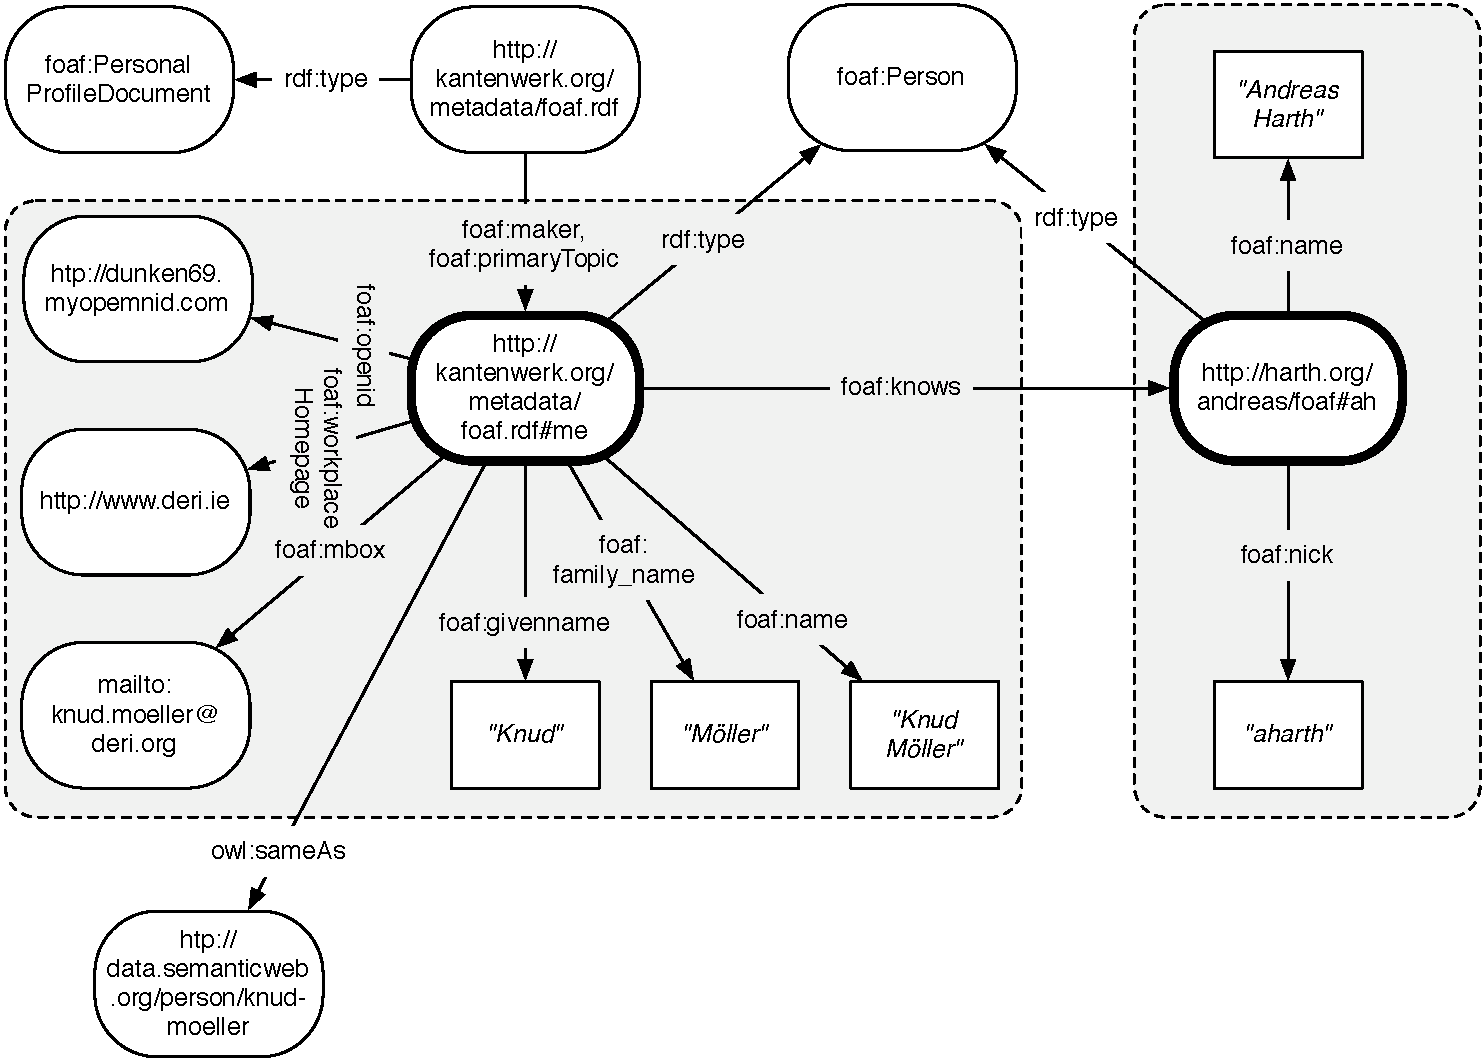
\includegraphics[width=\linewidth]{images/foaf_example.pdf}
    \caption{Example of FOAF data}
    \label{fig:foaf_example}
  \end{center}
\end{figure}

FOAF has been \emph{``evolving gradually since its creation in mid-2000''}~\cite{brickley2004foaf}. Over the years, it attracted a lot of attention and has become one of the major successes of the Semantic Web. Compared to most other ontologies or vocabularies, it has received a much higher uptake, with the number of FOAF files on the internet probably numbering tens of millions now. Its popularity in the community and beyond is also underlined by the fact that many other ontologies are integrating FOAF in order to represent basic information regarding people, or they are using it as a point of reference and extend the basic FOAF classes and properties for their own needs. Examples for this kind of integration are the increasingly popular SIOC (Semantically-Interlinked Online Communities) ontology~\cite{breslin2005communitiesEswc}, which uses FOAF description to unify identities in different online communities, or the Semantic Web Conference ontology~\cite{moeller2007dogfood}, where conference attendees or authors are represented as FOAF person instances.

The specification document of the FAST ontology defines that part of the purpose of the ontology is ``the description of users and user profiles''. The most obvious solution for implementing this requirement is to integrate the FAST ontology with FOAF. This means that each user of FAST would be modelled as a \texttt{foaf:Person}. A lot of the basic necessities in terms of user profile information is covered by properties defined in FOAF (names, contact details, interests, user pictures, etc.) and could therefore be used as is. In other cases, rather generic FOAF terms might be good starting points for extension towards more specific needs that occur in FAST. The icons of various components in the GVS may serve as an example here: the relation that holds between an icon and the thing X of which it is an icon could be described as ``the icon depicts X''. FOAF provides the property \texttt{depiction} to express this general relation. However, \texttt{hasIcon} (our property for saying that something is the icon of a thing) can be considered a specialisation of this, and so we will say that \texttt{fast:hasIcon} is a specialisation of \texttt{foaf:depiction}. In terms of RDFS, we will say that \texttt{<fast:hasIcon> <rdfs:subPropertyOf> <foaf:depiction>}.
% subsubsection foaf (end)

\subsubsection{SIOC} % (fold)
\label{ssub:sioc}

Another vocabulary that is gaining a lot of uptake and support on the Semantic Web is SIOC, which received additional weight when it became a W3C member submission in 2007. The basic idea behind SIOC is that there is an abstract model behind all online community sites which contain an aspect of discussion between members, be it forum sites, discussion boards, blogs, wikis, content management systems, mailing lists, etc. For each of those \emph{sites}, it can be said they contain discussion threads or \emph{fora}, which in turn contain \emph{posts}, which in turn can have \emph{comments}. Furthermore, each post or comment can have a \emph{topic} and a \emph{creator}, which can be a \emph{user} of the site. The authors of SIOC make a point of integrating the vocabulary with FOAF, e.g., by suggesting that a user of a site is in fact held by an instance of \texttt{foaf:Person} (the SIOC specification states that \texttt{sioc:User} is a sub-class of \texttt{foaf:OnlineAccount} \cite{sioc_spec2009}). An overview of the different classes and properties of SIOC is given in Fig.~\ref{fig:sioc_overview}.

\begin{figure}
  \begin{center}
    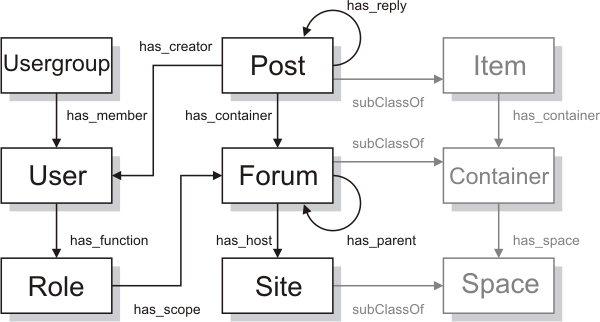
\includegraphics[width=\linewidth]{images/sioc_overview}
    \caption{Overview of the SIOC ontology}
    \label{fig:sioc_overview}
  \end{center}
\end{figure}

From an implementation point of view, a particular site will use SIOC by exposing its internal data on request with the help of a SIOC exporter. Such components have been provided by various members in the SIOC developer community for different popular platforms, such as the WordPress blogging software, the Drupal CMS or the Twitter micro-blogging platform. The benefit that sites are creating for end users by using SIOC is that a common representation format and reference points such as authors and topics allow data from different sites to be integrated and thus browsed and searched together.

From the point of view of the FAST gadget ontology, the most interesting features of the vocabulary are the classes and properties it provides for modelling users of a site. We will use SIOC in combination with FOAF to model users and their profiles, as well as user groups, as specified in the requirements document. The discussion aspects of SIOC will not have an immediate use within the FAST platform. However, it is conceivable that collaborative features such as support for fora will be added to FAST at some point, which will lead to an extension of the requirements document. These additional requirements could then be fulfilled by the integration of further terms from SIOC.
% subsubsection sioc (end)

\subsubsection{Dublin Core} % (fold)
\label{ssub:dublin_core}

Dublin Core (DC) is a set of metadata elements for describing online resources in order to support indexing, searching and finding them. Typical examples of terms from DC are \emph{title}, \emph{creator}, \emph{subject}, \emph{description}, \emph{date} or \emph{rights}. In principle, DC can be applied to a wide range of resources, but is typically used in the context of describing media (textual documents, video, sound or image). The initial work on DC was done at an invitational workshop in Dublin, Ohio, US (hence the name) in 1995. Since then, several revisions and extensions have been applied to the vocabulary.

While it is possible to express DC in plain HTML, the more widely used language is probably RDF. The original 15 terms were all properties defined in the DC elements namespace (\url{http://purl.org/dc/elements/1.1/}, short \texttt{dc}). The properties were not formally defined with respect to their range and domain, or whether they are object or datatype properties. However, the assumption was that the values for each property would always be literals, as opposed to complex values represented by a URI. More recently, the DC elements namespace has been declared legacy and is now superseded by the DC terms namespace (\url{http://purl.org/dc/terms/}, short \texttt{dcterms})~\cite{dcterms2008}, which includes more precise re-definitions of all 15 original terms, as well as a number of new terms (resulting in a total of 55 terms). This new iteration of DC now provides the facility to use structured values for properties and specifies what type these values will have. E.g., the property \texttt{dcterms:creator} now supersedes the original \texttt{dc:creator} and specifies that its value has the type \texttt{dcterms:Agent}.

In order to reconcile with the simplicity of the original, flat DC elements and the newer, more structured DC terms, DC also includes the so-called ``DumbDown'' principle, which basically says that structured values of DC terms should always carry a literal description as well, in order to cater for ``dumb'' agents processing the data. These literals should be expressed using properties such as \emph{rdfs:label} or \emph{rdf:value}.

Because of the open nature of the RDF model and the open-world assumption usually applied for RDFS and OWL, it is possible to integrate DC with other ontologies such as FOAF. E.g., it is possible and good practice to make a statement saying that the \texttt{dcterms:creator} of a document is an instance of \texttt{foaf:Person}. By inference following from the DC terms specification, this person would then also be a \texttt{dcterms:Agent}. This scenario is illustrated in Fig.~\ref{fig:dcterms_example}. A similar, but slightly out-dated example is given in \url{http://dublincore.org/documents/dcq-rdf-xml/}.

\begin{figure}
  \begin{center}
    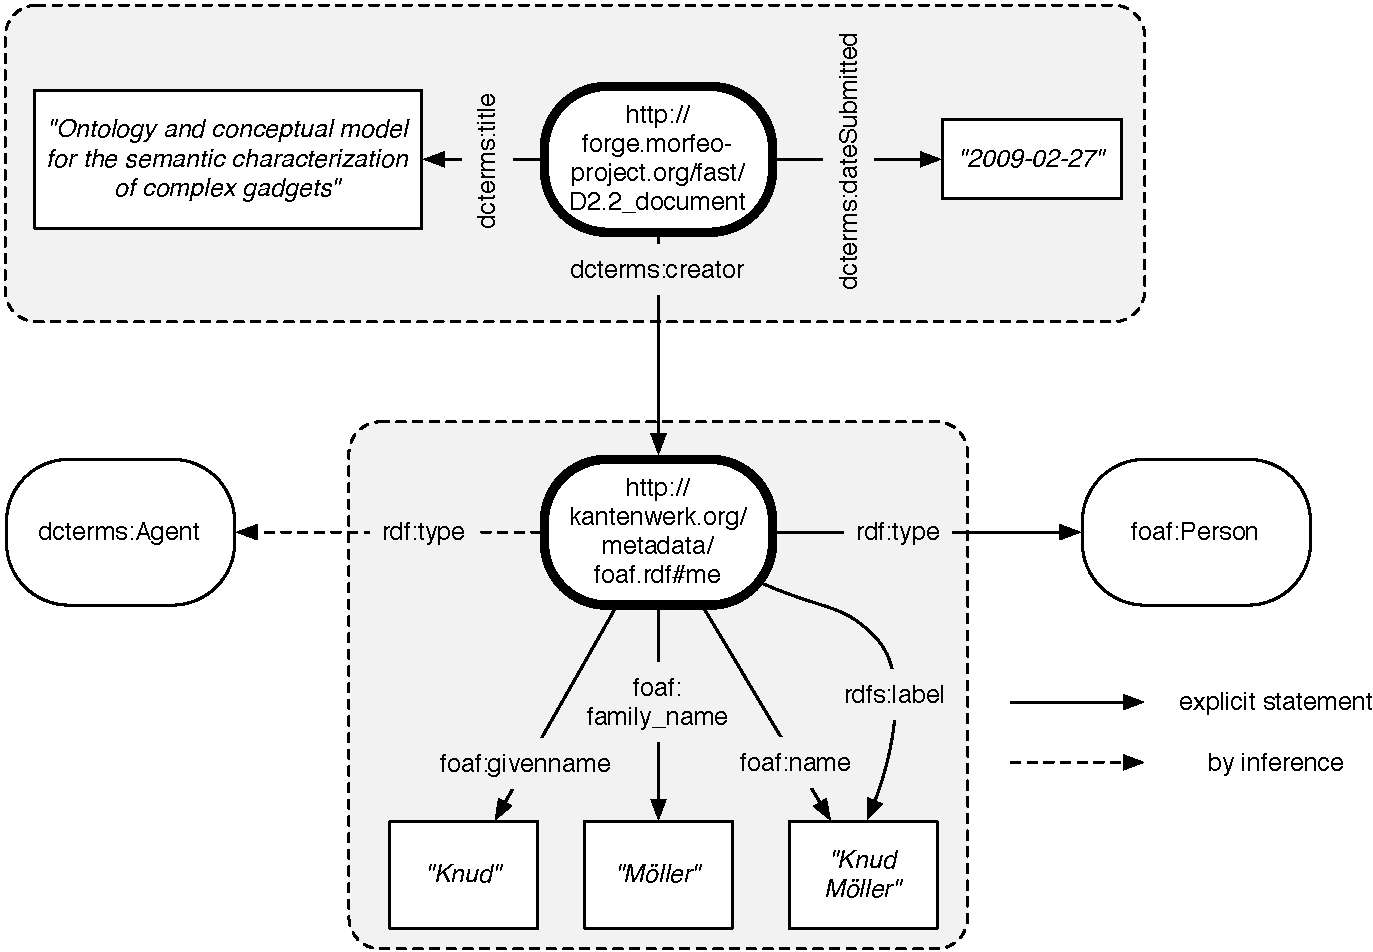
\includegraphics[width=\linewidth]{images/dcterms_example.pdf}
    \caption{Example of Dublin Core data}
    \label{fig:dcterms_example}
  \end{center}
\end{figure}


Looking at the requirements specification document, DC can be integrated into the FAST gadget ontology in many ways. A lot of the metadata needs for screens, screenflows and their components are identical to those of the media resources originally intended by DC. For this reason, many properties such as \texttt{title}, \texttt{creator}, \texttt{rights} or various \texttt{date} properties can be used directly (more details in the integration document). 
% subsubsection dublin_core (end)

\subsubsection{Common Tag} % (fold)
\label{ssub:common_tag}

Common Tag\footnote{\url{http://www.commontag.org}, 24/01/2010} is an open format and initiative for conceptual tagging, which is developed and backed by a number of relevant players in the Web community, including Yahoo! and DERI. The basic idea of conceptual tagging is to address the problem of ambiguity in the meaning of tags (e.g., does ``jaguar'' mean the car, the animal or the operating system?) as it occurs in free-text tagging. Rather than relying on methods such as clustering, applied to a whole corpus of tagged resources, conceptual tagging intends to disambiguate a tag right from the moment it is used, by linking it to an unambiguous concept from vocabularies such as DBpedia (representing Wikipedia as linked data) or Freebase. E.g., in order to disambiguate ``cocoa'' as meaning the API, not the drink or plant, it would be represented as a resource (rather than a plain literal) and linked to the DBpedia resource \url{http://dbpedia.org/resource/Cocoa_%28API%29}.

Apart from facilitating the disambiguation of tags, Common Tag also allows to make further assertions about the nature of a tag, such as who applied it or when it was applied. As an example, List.~\ref{list:common_tag} shows how a blog post has been tagged on 20/01/2010 with ``cocoa'', meaning the API, not the drink or plant.

\singlespacing
\lstset{
	caption={Common Tag example --- disambiguating the tag ``cocoa''}, 
	label=list:common_tag,
	language=turtle
}
\begin{figure}[ht]
	\lstinputlisting{exampleCode/common_tag_example.ttl}
\end{figure}
\doublespacing

Within FAST, Common Tag is used to cover the tagging needs as specified in the ontology requirements specification, and in particular in order to define the domain context as specified in the annotation part of the glossary of terms (\texttt{Tag} and \texttt{hasDomainContext}).

% subsubsection common_tag (end)

\subsubsection{Integration Document} % (fold)
\label{ssub:integration_document}
%
This living document specifies how the terms from the glossary of terms are expressed using terms from the various ontologies presented in the previous sections.

\singlespacing
\begin{small}
\begin{longtable}{|p{2.6cm}|p{1.5cm}|p{3cm}|p{7cm}|}
\caption{\label{tab:integration_document}FAST Ontology integration document}\\
\hline
\rowcolor{fast@lightgrey}\textcolor{white}{\textbf{FAST Term}} & 
\textcolor{white}{\textbf{Integrated Ontology}} & 
\textcolor{white}{\textbf{Integrated Term}} & 
\textcolor{white}{\textbf{Comment}} \\ \hline
\endfirsthead
\multicolumn{4}{|c|}{\emph{\textbf{Classes}}} \\ \hline
\texttt{User} & FOAF & \texttt{foaf:Person} & A user in FAST will be modelled using a combination of FOAF and SIOC, so that an instance of \texttt{foaf:Person} will have an account on the FAST platform, represented by an instance of \texttt{sioc:User}, which is a subclass of \texttt{foaf:OnlineAccount}. The relationship is expressed using \texttt{foaf:holdsAccount}. This way of modelling directly follows the suggestions made by~\cite{sioc_related2007}.\\ \hline
\texttt{User} & SIOC & \texttt{sioc:User} & s.a.\\ \hline
\texttt{Image} & FOAF & \texttt{foaf:Image} & --- \\ \hline
\texttt{Tag} & Common Tag & \texttt{ctag:Tag} & Complex or conceptual tags are being used e.g. to model the domain context of resources.	 \\ \hline
\multicolumn{4}{|c|}{\emph{\textbf{Properties}}} \\ \hline
\texttt{hasLabel} & DC & \texttt{dcterms:title} & ---  \\ \hline
\texttt{hasCreator} & DC & \texttt{dcterms:creator} & DC defines the range of \texttt{dcterms:creator} to be \texttt{dcterms:Agent}. By inference, this obviously also holds within FAST. However, we will explicitly only use \texttt{foaf:Person} (also see Fig.~\ref{fig:dcterms_example}). \\ \hline
\texttt{hasDescription} & DC & \texttt{dcterms:description} & --- \\ \hline
\texttt{hasCreationDate} & DC & \texttt{created} & Dates should be formatted according to ISO 8601. \\ \hline
\texttt{hasRights} & DC & \texttt{rights} & DC terms specify a number of classes to model the rights of resources. \texttt{dcterms:rights} links a resource to a \texttt{dcterms:RightsStatement}. The holder of the rights is specified by pointing from the resource to a \texttt{dcterms:Agent}, using the \texttt{dcterms:rightsHolder} property. \\ \hline
\texttt{hasDomainContext} & DC & \texttt{subject} & DC specifies that subject should be non-literals. To allow simple tagging, we should represent tags as resources (TODO). \\ \hline
\texttt{hasImage} & FOAF & \texttt{depiction} & The inverse \texttt{foaf:depicts} could also be used. \\ \hline
\texttt{hasName} & FOAF & \texttt{name} & Apart from \texttt{foaf:name}, which is used for the full name, more fine-grained properties such as \texttt{foaf:firstName}, \texttt{foaf:surname} or \texttt{foaf:title} and \texttt{foaf:nick} can be used as well. \\ \hline
\texttt{hasEmail} & FOAF & \texttt{mbox} & While \texttt{foaf:mbox} will be used for the plain e-mail address, \texttt{foaf:mbox\_sha1sum} will be used for an obfuscated version of the address. \\ \hline
\texttt{hasInterests} & FOAF & \texttt{foaf:interest} & --- \\ \hline
\texttt{hasUserName} & FOAF & \texttt{foaf:accountName} & --- \\ \hline
\texttt{hasDomainContext} & Common Tag & \texttt{ctag:tagged} & The domain context of a resource in FAST can be expressed as a complex tag. Further Common Tag properties can then be applied to make assertions about the tag itself. \\ \hline
\end{longtable}
\end{small}
\doublespacing

%% subsubsection integration_document (end)
%
%% subsection integration (end)
%
%% section domain_analysis (end)
%
\section{The FAST Gadget Ontology} % (fold)
\label{sec:ontology}

In the following sections we will define the FAST gadget ontology.

\subsection{Defining Pre- and Post-conditions} % (fold)
\label{sub:defining_pre_and_post_conditions}

The facts which define the pre- and post-conditions of screens and screenflows in FAST will be modelled as individual RDF triples. In effect, this means that conditions, which are sets of facts, can be modelled as graph patterns using SPARQL notation \cite{sparql2008spec}. E.g., a simple pre-condition such as \emph{``There has to be a user''} could be expressed as in List.~\ref{ex:simple_precondition}. Literally, this very simple pattern means \emph{``a variable ?user is of type sioc:User''}. In logical terms, it means something along the lines of \emph{``there exists a sioc:User''}. For the pre-condition to be fulfilled, it needs to be executed against the RDF graph in question (most likely the facts on the current canvas).

\singlespacing
\lstset{
	caption={Simple pre-condition}, 
	label=ex:simple_precondition,
	language=sparql
}
\begin{figure}[ht]
\begin{lstlisting}
	?user a sioc:User .
\end{lstlisting}
\end{figure}
\doublespacing

Post-conditions will be expressed in a similar fashion. At design time, post-condition patterns will have variable in the same way as pre-condition patterns. When a screen is added to the canvas, the pattern needs to be materialised. To do this, each variable will be replaced with a randomly generated URI or blank node. At runtime, variables will be replaced with actual values once the screen for which the post-condition holds has been executed. As an example, consider the post-condition of a login screen. In natural language, it could be \emph{``Once the login process has finished, there will be a user object''}. Using the same notation as before, this could be expressed as shown in List.~\ref{ex:postcondition}, extended with some additional facts (\emph{``There is a user object which has an account name. There is also a person which has a name, and which has the user object as an online account.''}).

\singlespacing
\lstset{
	caption={Simple post-condition}, 
	label=ex:postcondition,
	language=sparql
}
\begin{figure}[ht]
\begin{lstlisting}
	?user a sioc:User ;
	      foaf:accountName ?account_name .
	?person a foaf:Person ;
	      foaf:holdsAccount ?user ;
	      foaf:name ?person_name .
\end{lstlisting}
\end{figure}
\doublespacing

Once added to the canvas in the GVS (``instantiated at design time''), each variable would be replaced with a blank node identifier, as shown in example~\ref{ex:postcondition_canvas}. The pre-condition in example~\ref{ex:simple_precondition} could now be executed successfully as a SPARQL query against the canvas graph.

\singlespacing
\lstset{
	caption={Post-condition on the FAST GVS canvas}, 
	label=ex:postcondition_canvas,
	language=sparql
}
\begin{figure}[ht]
\begin{lstlisting}
	_:b0 a sioc:User ;
	      foaf:accountName _:b1 .
	_:b2 a foaf:Person ;
	      foaf:holdsAccount _:b0 ;
	      foaf:name _:b3 .
\end{lstlisting}
\end{figure}
\doublespacing

Finally, during runtime, the post-condition's variables would be replaced with the actual values of the user which completed the login screen (``instantiated during runtime''). E.g., this could result in a graph such as in example~\ref{ex:postcondition_runtime}.

\singlespacing
\lstset{
	caption={Post-condition during runtime}, 
	label=ex:postcondition_runtime,
	language=sparql
}
\begin{figure}[ht]
\begin{lstlisting}
	<http://fast.org/gvs/knud> a sioc:User ;
	      foaf:accountName "dunk" .
	<http://kantenwerk.org/metadata/foaf.rdf#me> a foaf:Person ;
	      foaf:holdsAccount <http://fast.org/gvs/knud> ;
	      foaf:name "Knud Moeller" .
\end{lstlisting}
\end{figure}
\doublespacing


Since graph patterns with variable cannot directly be expressed in RDF (short of using blank nodes, which cannot have labels), the graph patterns are expressed as RDF literals and linked \texttt{fast:Condition} instances using the \texttt{fast:hasPattern} property.
Each such condition will be linked to a screen or screenflow using either the \texttt{fast:hasPreCondition} or \texttt{fast:hasPostCondition} property.

Since SPARQL has no direct support for negation, and since there is a need to allow screens to remove facts from the canvas graph as well as adding them, both pre- and post-conditions can be modelled to be either \emph{positive} or \emph{negative} using the \texttt{fast:isPositive} property. For pre-conditions, the interpretation of \emph{positive} is that the condition must hold, while \emph{negative} means that the negation of the condition must hold. For post-conditions, \emph{positive} leads to the instantiated condition being added to the canvas, while \emph{negative} will remove the instantiated condition. These interpretations are summarised in Tab.~\ref{tab:is_positive}.

\begin{table}[h]
\caption{Different semantics for \texttt{isPositive}}
\label{tab:is_positive}
\begin{center}
\begin{tabular}{|l|c|c|}
\hline
& pre-condition & post-condition \\ \hline
\emph{isPositive ``YES''} & condition must be fulfilled & condition instantiated\\ \hline
\emph{isPositive ``NO''} & $\neg$condition must be fulfilled & instantiated condition removed \\ \hline
\end{tabular}
\end{center}
\end{table}

\subsection{Instance Examples} % (fold)
\label{sub:instance_examples}

\subsubsection{Complete Screen with Opaque Code} % (fold)
\label{ssub:complete_screen}

\singlespacing
\lstset{
	caption={Complete Screen with Opaque Code}, 
	label=list:screen_01
}
% \setlength\parindent{0in}
% \begin{minipage}[t]{\textwidth}
\lstinputlisting{exampleCode/01_screenExample.ttl}
% \end{minipage}
% \setlength\parindent{0.21in}
\doublespacing

% subsubsection complete_screen (end)

\subsubsection{Complete Screen with Declarative Definition} % (fold)
\label{ssub:complete_screen_with_declarative_definition}

\singlespacing
\lstset{
	caption={Complete Screen with Declarative Definition}, 
	label=list:screen_01
}
% \setlength\parindent{0in}
% \begin{minipage}[t]{\textwidth}
\lstinputlisting{exampleCode/02_screenExample.ttl}
% \end{minipage}
% \setlength\parindent{0.21in}
\doublespacing
% subsubsection complete_screen_with_declarative_definition (end)

% subsection instance_examples (end)


\subsection{Classes} % (fold)
\label{sub:classes}

This section contains a definition of all classes defined in the \texttt{fgo} namespace. For classes integrated from other ontologies, see the integration document~\ref{ssub:integration_document}.

\singlespacing
\begin{small}
\subsubsection*{Class: \texttt{fgo:Action}}
\label{subs:Action}
\begin{tabular}{| >{\columncolor{fast@lightgrey}}p{2.5cm}|p{12cm}|}
\hline
\textcolor{white}{\textbf{label}} & Action \\ \hline
\textcolor{white}{\textbf{description}} & An action represents a specific routine which will be performed when a certain
condition is fulfilled within a certain screen component. Examples are methods of a Web service (e.g., getItem) or functionality to update or change the contents of a form. \\ \hline
\textcolor{white}{\textbf{sub\_class\_of}} & \htmlref{\texttt{fgo:BuildingBlock}}{subs:BuildingBlock} \\ \hline
\textcolor{white}{\textbf{in\_domain\_of}} & \htmlref{\texttt{fgo:hasUse}}{subs:hasUse} \\ \hline
\textcolor{white}{\textbf{in\_range\_of}} & \htmlref{\texttt{fgo:hasAction}}{subs:hasAction} \\ \hline
\end{tabular}
\subsubsection*{Class: \texttt{fgo:BackendService}}
\label{subs:BackendService}
\begin{tabular}{| >{\columncolor{fast@lightgrey}}p{2.5cm}|p{12cm}|}
\hline
\textcolor{white}{\textbf{label}} & Backend Service \\ \hline
\textcolor{white}{\textbf{description}} & A Web service which provides data and/or functionality to a screen. The actual backend service is external to FAST, and only available through a wrapper (the service Resource). \\ \hline
\textcolor{white}{\textbf{sub\_class\_of}} & \htmlref{\texttt{fgo:BuildingBlock}}{subs:BuildingBlock} \\ \hline
\end{tabular}
\subsubsection*{Class: \texttt{fgo:BuildingBlock}}
\label{subs:BuildingBlock}
\begin{tabular}{| >{\columncolor{fast@lightgrey}}p{2.5cm}|p{12cm}|}
\hline
\textcolor{white}{\textbf{label}} & BuildingBlock \\ \hline
\textcolor{white}{\textbf{description}} & Anything that is part of a gadget. Tentatively anything that can be `touched' and moved around in the FAST IDE, from the most complex units such as screen flows, down to atomic form elements like a button or a label in a form. \\ \hline
\textcolor{white}{\textbf{super\_class\_of}} & \htmlref{\texttt{fgo:Action}}{subs:Action}, \htmlref{\texttt{fgo:BackendService}}{subs:BackendService}, \htmlref{\texttt{fgo:Condition}}{subs:Condition}, \htmlref{\texttt{fgo:Fact}}{subs:Fact}, \htmlref{\texttt{fgo:FormElement}}{subs:FormElement}, \htmlref{\texttt{fgo:Library}}{subs:Library}, \htmlref{\texttt{fgo:Pipe}}{subs:Pipe}, \htmlref{\texttt{fgo:Screen}}{subs:Screen}, \htmlref{\texttt{fgo:ScreenComponent}}{subs:ScreenComponent}, \htmlref{\texttt{fgo:ScreenFlow}}{subs:ScreenFlow}, \htmlref{\texttt{fgo:Trigger}}{subs:Trigger} \\ \hline
\textcolor{white}{\textbf{in\_domain\_of}} & \htmlref{\texttt{fgo:contains}}{subs:contains}, \htmlref{\texttt{fgo:hasIcon}}{subs:hasIcon}, \htmlref{\texttt{fgo:hasScreenshot}}{subs:hasScreenshot} \\ \hline
\textcolor{white}{\textbf{in\_range\_of}} & \htmlref{\texttt{fgo:contains}}{subs:contains} \\ \hline
\end{tabular}
\subsubsection*{Class: \texttt{fgo:Condition}}
\label{subs:Condition}
\begin{tabular}{| >{\columncolor{fast@lightgrey}}p{2.5cm}|p{12cm}|}
\hline
\textcolor{white}{\textbf{label}} & Condition \\ \hline
\textcolor{white}{\textbf{description}} & The pre- or post-condition of a certain kinds of building block. If the building block is a screen flow, each target platform will use these conditions in its own way, or may also ignore them. E.g., in EzWeb pre- and post-conditions correspond to the concepts of slot and event.
A condition can be seen as a RDF bag of facts, where every fact has to be true
for the condition be true as well. \\ \hline
\textcolor{white}{\textbf{sub\_class\_of}} & \htmlref{\texttt{fgo:BuildingBlock}}{subs:BuildingBlock} \\ \hline
\textcolor{white}{\textbf{in\_range\_of}} & \htmlref{\texttt{fgo:hasPostCondition}}{subs:hasPostCondition}, \htmlref{\texttt{fgo:hasPreCondition}}{subs:hasPreCondition} \\ \hline
\end{tabular}
\subsubsection*{Class: \texttt{fgo:Fact}}
\label{subs:Fact}
\begin{tabular}{| >{\columncolor{fast@lightgrey}}p{2.5cm}|p{12cm}|}
\hline
\textcolor{white}{\textbf{label}} & Fact \\ \hline
\textcolor{white}{\textbf{description}} & The `basic information unit of a FAST gadget'. In terms of RDF, a fact is a statement consisting of a subject, predicate and object (S, P, O). \\ \hline
\textcolor{white}{\textbf{sub\_class\_of}} & \htmlref{\texttt{fgo:BuildingBlock}}{subs:BuildingBlock} \\ \hline
\textcolor{white}{\textbf{in\_domain\_of}} & \htmlref{\texttt{fgo:hasPattern}}{subs:hasPattern}, \htmlref{\texttt{fgo:hasPatternString}}{subs:hasPatternString}, \htmlref{\texttt{fgo:isPositive}}{subs:isPositive} \\ \hline
\end{tabular}
\subsubsection*{Class: \texttt{fgo:Form}}
\label{subs:Form}
\begin{tabular}{| >{\columncolor{fast@lightgrey}}p{2.5cm}|p{12cm}|}
\hline
\textcolor{white}{\textbf{label}} & Form \\ \hline
\textcolor{white}{\textbf{description}} & A form is the visual aspect of a screen: its user interface. Each form is made up of individual form elements. \\ \hline
\textcolor{white}{\textbf{sub\_class\_of}} & \htmlref{\texttt{fgo:ScreenComponent}}{subs:ScreenComponent} \\ \hline
\textcolor{white}{\textbf{in\_domain\_of}} & \htmlref{\texttt{fgo:hasFormElement}}{subs:hasFormElement} \\ \hline
\textcolor{white}{\textbf{in\_range\_of}} & \htmlref{\texttt{fgo:hasForm}}{subs:hasForm} \\ \hline
\end{tabular}
\subsubsection*{Class: \texttt{fgo:FormElement}}
\label{subs:FormElement}
\begin{tabular}{| >{\columncolor{fast@lightgrey}}p{2.5cm}|p{12cm}|}
\hline
\textcolor{white}{\textbf{label}} & Form Element \\ \hline
\textcolor{white}{\textbf{description}} & Form elements are UI elements in a particular screen, such as buttons, lists or labels. \\ \hline
\textcolor{white}{\textbf{sub\_class\_of}} & \htmlref{\texttt{fgo:BuildingBlock}}{subs:BuildingBlock} \\ \hline
\textcolor{white}{\textbf{in\_range\_of}} & \htmlref{\texttt{fgo:hasFormElement}}{subs:hasFormElement} \\ \hline
\end{tabular}
\subsubsection*{Class: \texttt{fgo:Library}}
\label{subs:Library}
\begin{tabular}{| >{\columncolor{fast@lightgrey}}p{2.5cm}|p{12cm}|}
\hline
\textcolor{white}{\textbf{label}} & Library \\ \hline
\textcolor{white}{\textbf{description}} & Libraries are references to external code libraries required for the execution of a particular building block at runtime. \\ \hline
\textcolor{white}{\textbf{sub\_class\_of}} & \htmlref{\texttt{fgo:BuildingBlock}}{subs:BuildingBlock} \\ \hline
\textcolor{white}{\textbf{in\_domain\_of}} & \htmlref{\texttt{fgo:hasLanguage}}{subs:hasLanguage} \\ \hline
\textcolor{white}{\textbf{in\_range\_of}} & \htmlref{\texttt{fgo:hasLibrary}}{subs:hasLibrary} \\ \hline
\end{tabular}
\subsubsection*{Class: \texttt{fgo:Operator}}
\label{subs:Operator}
\begin{tabular}{| >{\columncolor{fast@lightgrey}}p{2.5cm}|p{12cm}|}
\hline
\textcolor{white}{\textbf{label}} & Operator \\ \hline
\textcolor{white}{\textbf{description}} & Operators are intended to transform and/or modify data within a screen, usually for preparing data coming from service resources for the use in the screen's interface. Operators cover different kinds of data manipulations, from simple aggregation to mediating data with incompatible schemas. \\ \hline
\textcolor{white}{\textbf{sub\_class\_of}} & \htmlref{\texttt{fgo:ScreenComponent}}{subs:ScreenComponent} \\ \hline
\textcolor{white}{\textbf{in\_range\_of}} & \htmlref{\texttt{fgo:hasOperator}}{subs:hasOperator} \\ \hline
\end{tabular}
\subsubsection*{Class: \texttt{fgo:Pipe}}
\label{subs:Pipe}
\begin{tabular}{| >{\columncolor{fast@lightgrey}}p{2.5cm}|p{12cm}|}
\hline
\textcolor{white}{\textbf{label}} & pipe or connector \\ \hline
\textcolor{white}{\textbf{description}} & Pipes are used to explicitly define the flow of data within a screen, e.g., from service resource to operator to a specific form element. \\ \hline
\textcolor{white}{\textbf{sub\_class\_of}} & \htmlref{\texttt{fgo:BuildingBlock}}{subs:BuildingBlock} \\ \hline
\textcolor{white}{\textbf{in\_domain\_of}} & \htmlref{\texttt{fgo:hasIdActionTo}}{subs:hasIdActionTo}, \htmlref{\texttt{fgo:hasIdBBFrom}}{subs:hasIdBBFrom}, \htmlref{\texttt{fgo:hasIdBBTo}}{subs:hasIdBBTo}, \htmlref{\texttt{fgo:hasIdConditionFrom}}{subs:hasIdConditionFrom}, \htmlref{\texttt{fgo:hasIdConditionTo}}{subs:hasIdConditionTo} \\ \hline
\end{tabular}
\subsubsection*{Class: \texttt{fgo:Resource}}
\label{subs:Resource}
\begin{tabular}{| >{\columncolor{fast@lightgrey}}p{2.5cm}|p{12cm}|}
\hline
\textcolor{white}{\textbf{label}} & Resource \\ \hline
\textcolor{white}{\textbf{description}} & A service resource in FAST is a wrapper around a Web service (the backend service), which makes the service available to the platform, e.g., by mapping its definition to FAST facts and actions. \\ \hline
\textcolor{white}{\textbf{sub\_class\_of}} & \htmlref{\texttt{fgo:ScreenComponent}}{subs:ScreenComponent} \\ \hline
\textcolor{white}{\textbf{in\_range\_of}} & \htmlref{\texttt{fgo:hasResource}}{subs:hasResource} \\ \hline
\end{tabular}
\subsubsection*{Class: \texttt{fgo:Screen}}
\label{subs:Screen}
\begin{tabular}{| >{\columncolor{fast@lightgrey}}p{2.5cm}|p{12cm}|}
\hline
\textcolor{white}{\textbf{label}} & Screen \\ \hline
\textcolor{white}{\textbf{description}} & An individual screen; the basic unit of user interaction in FAST. A screen is the interface through which a user gets access to data and functionality of a backend service. \\ \hline
\textcolor{white}{\textbf{sub\_class\_of}} & \htmlref{\texttt{fgo:BuildingBlock}}{subs:BuildingBlock} \\ \hline
\textcolor{white}{\textbf{in\_domain\_of}} & \htmlref{\texttt{fgo:hasForm}}{subs:hasForm}, \htmlref{\texttt{fgo:hasOperator}}{subs:hasOperator}, \htmlref{\texttt{fgo:hasResource}}{subs:hasResource} \\ \hline
\end{tabular}
\subsubsection*{Class: \texttt{fgo:ScreenComponent}}
\label{subs:ScreenComponent}
\begin{tabular}{| >{\columncolor{fast@lightgrey}}p{2.5cm}|p{12cm}|}
\hline
\textcolor{white}{\textbf{label}} & Screen Component \\ \hline
\textcolor{white}{\textbf{description}} & Screens are made up of screen components, which fundamentally include service resources, operators and forms. \\ \hline
\textcolor{white}{\textbf{super\_class\_of}} & \htmlref{\texttt{fgo:Form}}{subs:Form}, \htmlref{\texttt{fgo:Operator}}{subs:Operator}, \htmlref{\texttt{fgo:Resource}}{subs:Resource} \\ \hline
\textcolor{white}{\textbf{sub\_class\_of}} & \htmlref{\texttt{fgo:BuildingBlock}}{subs:BuildingBlock} \\ \hline
\textcolor{white}{\textbf{in\_domain\_of}} & \htmlref{\texttt{fgo:hasAction}}{subs:hasAction}, \htmlref{\texttt{fgo:hasTrigger}}{subs:hasTrigger} \\ \hline
\end{tabular}
\subsubsection*{Class: \texttt{fgo:ScreenFlow}}
\label{subs:ScreenFlow}
\begin{tabular}{| >{\columncolor{fast@lightgrey}}p{2.5cm}|p{12cm}|}
\hline
\textcolor{white}{\textbf{label}} & Screen Flow \\ \hline
\textcolor{white}{\textbf{description}} & A set of screens from which a gadget for a given target platform can be generated. \\ \hline
\textcolor{white}{\textbf{sub\_class\_of}} & \htmlref{\texttt{fgo:BuildingBlock}}{subs:BuildingBlock} \\ \hline
\end{tabular}
\subsubsection*{Class: \texttt{fgo:Trigger}}
\label{subs:Trigger}
\begin{tabular}{| >{\columncolor{fast@lightgrey}}p{2.5cm}|p{12cm}|}
\hline
\textcolor{white}{\textbf{label}} & Trigger \\ \hline
\textcolor{white}{\textbf{description}} & Triggers are the flip-side of actions. Certain events in a building block can cause a trigger to be fired. Other building blocks within the same screen, which are listening to it, will react with an action. \\ \hline
\textcolor{white}{\textbf{sub\_class\_of}} & \htmlref{\texttt{fgo:BuildingBlock}}{subs:BuildingBlock} \\ \hline
\textcolor{white}{\textbf{in\_domain\_of}} & \htmlref{\texttt{fgo:hasIdActionTo}}{subs:hasIdActionTo}, \htmlref{\texttt{fgo:hasIdBBFrom}}{subs:hasIdBBFrom}, \htmlref{\texttt{fgo:hasIdBBTo}}{subs:hasIdBBTo}, \htmlref{\texttt{fgo:hasNameFrom}}{subs:hasNameFrom} \\ \hline
\textcolor{white}{\textbf{in\_range\_of}} & \htmlref{\texttt{fgo:hasTrigger}}{subs:hasTrigger} \\ \hline
\end{tabular}
\subsubsection*{Class: \texttt{fgo:WithCode}}
\label{subs:WithCode}
\begin{tabular}{| >{\columncolor{fast@lightgrey}}p{2.5cm}|p{12cm}|}
\hline
\textcolor{white}{\textbf{label}} & With Code \\ \hline
\textcolor{white}{\textbf{description}} & Any kind of building block that can be defined as a whole through code. \\ \hline
\textcolor{white}{\textbf{in\_domain\_of}} & \htmlref{\texttt{fgo:hasCode}}{subs:hasCode}, \htmlref{\texttt{fgo:hasLibrary}}{subs:hasLibrary} \\ \hline
\textcolor{white}{\textbf{unionOf}} & \htmlref{\texttt{fgo:Form}}{subs:Form}, \htmlref{\texttt{fgo:Operator}}{subs:Operator}, \htmlref{\texttt{fgo:Resource}}{subs:Resource}, \htmlref{\texttt{fgo:Screen}}{subs:Screen} \\ \hline
\end{tabular}
\subsubsection*{Class: \texttt{fgo:WithDefinition}}
\label{subs:WithDefinition}
\begin{tabular}{| >{\columncolor{fast@lightgrey}}p{2.5cm}|p{12cm}|}
\hline
\textcolor{white}{\textbf{label}} & With Definition \\ \hline
\textcolor{white}{\textbf{description}} & Any kind of building block that can be defined declaratively in the GVS. \\ \hline
\textcolor{white}{\textbf{unionOf}} & \htmlref{\texttt{fgo:Form}}{subs:Form}, \htmlref{\texttt{fgo:Screen}}{subs:Screen} \\ \hline
\end{tabular}
\subsubsection*{Class: \texttt{fgo:WithPostConditions}}
\label{subs:WithPostConditions}
\begin{tabular}{| >{\columncolor{fast@lightgrey}}p{2.5cm}|p{12cm}|}
\hline
\textcolor{white}{\textbf{label}} & With Post-condition \\ \hline
\textcolor{white}{\textbf{description}} & Those kinds of building blocks which can have post-conditions. \\ \hline
\textcolor{white}{\textbf{in\_domain\_of}} & \htmlref{\texttt{fgo:hasPostCondition}}{subs:hasPostCondition} \\ \hline
\textcolor{white}{\textbf{unionOf}} & \htmlref{\texttt{fgo:Screen}}{subs:Screen}, \htmlref{\texttt{fgo:ScreenComponent}}{subs:ScreenComponent}, \htmlref{\texttt{fgo:ScreenFlow}}{subs:ScreenFlow} \\ \hline
\end{tabular}
\subsubsection*{Class: \texttt{fgo:WithPreConditions}}
\label{subs:WithPreConditions}
\begin{tabular}{| >{\columncolor{fast@lightgrey}}p{2.5cm}|p{12cm}|}
\hline
\textcolor{white}{\textbf{label}} & With Pre-condition \\ \hline
\textcolor{white}{\textbf{description}} & Those kinds of building blocks which can have pre-conditions. \\ \hline
\textcolor{white}{\textbf{in\_domain\_of}} & \htmlref{\texttt{fgo:hasPreCondition}}{subs:hasPreCondition} \\ \hline
\textcolor{white}{\textbf{unionOf}} & \htmlref{\texttt{fgo:Action}}{subs:Action}, \htmlref{\texttt{fgo:Screen}}{subs:Screen}, \htmlref{\texttt{fgo:ScreenFlow}}{subs:ScreenFlow} \\ \hline
\end{tabular}

\end{small}
\doublespacing

%subsection classes (end)

\subsection{Properties} % (fold)
\label{sub:properties}

This section contains a definition of all properties defined in the \texttt{fgo} namespace. For properties integrated from other ontologies, see the integration document~\ref{ssub:integration_document}.

\singlespacing
\begin{small}
\subsubsection*{Property: \texttt{fgo:contains}}
\label{subs:contains}
\begin{tabular}{| >{\columncolor{fast@lightgrey}}p{2.5cm}|p{12cm}|}
\hline
\textcolor{white}{\textbf{label}} & contains \\ \hline
\textcolor{white}{\textbf{description}} & Many kinds of components in FAST can contain other components: 
screenflows contain screens, screens contain forms or form elements, etc.
It points to a resource reference to give a unique `id' to each component
within the resource. \\ \hline
\textcolor{white}{\textbf{type}} & \texttt{owl:ObjectProperty} \\ \hline
\textcolor{white}{\textbf{domain}} & \htmlref{\texttt{fgo:BuildingBlock}}{subs:BuildingBlock} \\ \hline
\textcolor{white}{\textbf{range}} & \htmlref{\texttt{fgo:BuildingBlock}}{subs:BuildingBlock} \\ \hline
\end{tabular}
\subsubsection*{Property: \texttt{fgo:hasAction}}
\label{subs:hasAction}
\begin{tabular}{| >{\columncolor{fast@lightgrey}}p{2.5cm}|p{12cm}|}
\hline
\textcolor{white}{\textbf{label}} & has action \\ \hline
\textcolor{white}{\textbf{description}} & This property indicates which actions are associated and can be perfomed within 
a screen component. \\ \hline
\textcolor{white}{\textbf{type}} & \texttt{owl:ObjectProperty} \\ \hline
\textcolor{white}{\textbf{domain}} & \htmlref{\texttt{fgo:ScreenComponent}}{subs:ScreenComponent} \\ \hline
\textcolor{white}{\textbf{range}} & \htmlref{\texttt{fgo:Action}}{subs:Action} \\ \hline
\end{tabular}
\subsubsection*{Property: \texttt{fgo:hasCode}}
\label{subs:hasCode}
\begin{tabular}{| >{\columncolor{fast@lightgrey}}p{2.5cm}|p{12cm}|}
\hline
\textcolor{white}{\textbf{label}} & has code \\ \hline
\textcolor{white}{\textbf{description}} & URL of the executable code of a particular building block (currently screens or screen components). \\ \hline
\textcolor{white}{\textbf{type}} & \texttt{owl:ObjectProperty} \\ \hline
\textcolor{white}{\textbf{domain}} & \htmlref{\texttt{fgo:WithCode}}{subs:WithCode} \\ \hline
\textcolor{white}{\textbf{range}} & \texttt{foaf:Document} \\ \hline
\end{tabular}
\subsubsection*{Property: \texttt{fgo:hasForm}}
\label{subs:hasForm}
\begin{tabular}{| >{\columncolor{fast@lightgrey}}p{2.5cm}|p{12cm}|}
\hline
\textcolor{white}{\textbf{label}} & has form \\ \hline
\textcolor{white}{\textbf{description}} & If a screen is defined declaratively, this property links it to its form (i.e., its visual user interface). \\ \hline
\textcolor{white}{\textbf{type}} & \texttt{owl:ObjectProperty} \\ \hline
\textcolor{white}{\textbf{domain}} & \htmlref{\texttt{fgo:Screen}}{subs:Screen} \\ \hline
\textcolor{white}{\textbf{range}} & \htmlref{\texttt{fgo:Form}}{subs:Form} \\ \hline
\end{tabular}
\subsubsection*{Property: \texttt{fgo:hasFormElement}}
\label{subs:hasFormElement}
\begin{tabular}{| >{\columncolor{fast@lightgrey}}p{2.5cm}|p{12cm}|}
\hline
\textcolor{white}{\textbf{label}} & has form element \\ \hline
\textcolor{white}{\textbf{description}} & If a form is defined declaratively, its elements are linked to it with this property. \\ \hline
\textcolor{white}{\textbf{type}} & \texttt{owl:ObjectProperty} \\ \hline
\textcolor{white}{\textbf{domain}} & \htmlref{\texttt{fgo:Form}}{subs:Form} \\ \hline
\textcolor{white}{\textbf{range}} & \htmlref{\texttt{fgo:FormElement}}{subs:FormElement} \\ \hline
\end{tabular}
\subsubsection*{Property: \texttt{fgo:hasIcon}}
\label{subs:hasIcon}
\begin{tabular}{| >{\columncolor{fast@lightgrey}}p{2.5cm}|p{12cm}|}
\hline
\textcolor{white}{\textbf{label}} & has icon \\ \hline
\textcolor{white}{\textbf{description}} & A small graphical representation of any FAST component or sub-component. \\ \hline
\textcolor{white}{\textbf{type}} & \texttt{owl:ObjectProperty} \\ \hline
\textcolor{white}{\textbf{domain}} & \htmlref{\texttt{fgo:BuildingBlock}}{subs:BuildingBlock} \\ \hline
\textcolor{white}{\textbf{range}} & \texttt{foaf:Image} \\ \hline
\end{tabular}
\subsubsection*{Property: \texttt{fgo:hasIdActionTo}}
\label{subs:hasIdActionTo}
\begin{tabular}{| >{\columncolor{fast@lightgrey}}p{2.5cm}|p{12cm}|}
\hline
\textcolor{white}{\textbf{label}} & has id action to \\ \hline
\textcolor{white}{\textbf{description}} & action id of the `to' point of the pipe or trigger. \\ \hline
\textcolor{white}{\textbf{type}} & \texttt{owl:DatatypeProperty} \\ \hline
\textcolor{white}{\textbf{domain}} & \htmlref{\texttt{fgo:Pipe}}{subs:Pipe}, \htmlref{\texttt{fgo:Trigger}}{subs:Trigger} \\ \hline
\textcolor{white}{\textbf{range}} & \texttt{xsd:string} \\ \hline
\end{tabular}
\subsubsection*{Property: \texttt{fgo:hasIdBBFrom}}
\label{subs:hasIdBBFrom}
\begin{tabular}{| >{\columncolor{fast@lightgrey}}p{2.5cm}|p{12cm}|}
\hline
\textcolor{white}{\textbf{label}} & has id building block from \\ \hline
\textcolor{white}{\textbf{description}} & building block id of the `from' point of the pipe or trigger. \\ \hline
\textcolor{white}{\textbf{type}} & \texttt{owl:DatatypeProperty} \\ \hline
\textcolor{white}{\textbf{domain}} & \htmlref{\texttt{fgo:Pipe}}{subs:Pipe}, \htmlref{\texttt{fgo:Trigger}}{subs:Trigger} \\ \hline
\textcolor{white}{\textbf{range}} & \texttt{xsd:string} \\ \hline
\end{tabular}
\subsubsection*{Property: \texttt{fgo:hasIdBBTo}}
\label{subs:hasIdBBTo}
\begin{tabular}{| >{\columncolor{fast@lightgrey}}p{2.5cm}|p{12cm}|}
\hline
\textcolor{white}{\textbf{label}} & has id building block to \\ \hline
\textcolor{white}{\textbf{description}} & building block id of the `to' point of the pipe or trigger. \\ \hline
\textcolor{white}{\textbf{type}} & \texttt{owl:DatatypeProperty} \\ \hline
\textcolor{white}{\textbf{domain}} & \htmlref{\texttt{fgo:Pipe}}{subs:Pipe}, \htmlref{\texttt{fgo:Trigger}}{subs:Trigger} \\ \hline
\textcolor{white}{\textbf{range}} & \texttt{xsd:string} \\ \hline
\end{tabular}
\subsubsection*{Property: \texttt{fgo:hasIdConditionFrom}}
\label{subs:hasIdConditionFrom}
\begin{tabular}{| >{\columncolor{fast@lightgrey}}p{2.5cm}|p{12cm}|}
\hline
\textcolor{white}{\textbf{label}} & has id condition from \\ \hline
\textcolor{white}{\textbf{description}} & condition id of the `from' point of the pipe. \\ \hline
\textcolor{white}{\textbf{type}} & \texttt{owl:DatatypeProperty} \\ \hline
\textcolor{white}{\textbf{domain}} & \htmlref{\texttt{fgo:Pipe}}{subs:Pipe} \\ \hline
\textcolor{white}{\textbf{range}} & \texttt{xsd:string} \\ \hline
\end{tabular}
\subsubsection*{Property: \texttt{fgo:hasIdConditionTo}}
\label{subs:hasIdConditionTo}
\begin{tabular}{| >{\columncolor{fast@lightgrey}}p{2.5cm}|p{12cm}|}
\hline
\textcolor{white}{\textbf{label}} & has id condition to \\ \hline
\textcolor{white}{\textbf{description}} & condition id of the `to' point of the pipe. \\ \hline
\textcolor{white}{\textbf{type}} & \texttt{owl:DatatypeProperty} \\ \hline
\textcolor{white}{\textbf{domain}} & \htmlref{\texttt{fgo:Pipe}}{subs:Pipe} \\ \hline
\textcolor{white}{\textbf{range}} & \texttt{xsd:string} \\ \hline
\end{tabular}
\subsubsection*{Property: \texttt{fgo:hasLanguage}}
\label{subs:hasLanguage}
\begin{tabular}{| >{\columncolor{fast@lightgrey}}p{2.5cm}|p{12cm}|}
\hline
\textcolor{white}{\textbf{label}} & has language string \\ \hline
\textcolor{white}{\textbf{description}} & This property is the language the library is written in. \\ \hline
\textcolor{white}{\textbf{type}} & \texttt{owl:DatatypeProperty} \\ \hline
\textcolor{white}{\textbf{domain}} & \htmlref{\texttt{fgo:Library}}{subs:Library} \\ \hline
\textcolor{white}{\textbf{range}} & \texttt{xsd:string} \\ \hline
\end{tabular}
\subsubsection*{Property: \texttt{fgo:hasLibrary}}
\label{subs:hasLibrary}
\begin{tabular}{| >{\columncolor{fast@lightgrey}}p{2.5cm}|p{12cm}|}
\hline
\textcolor{white}{\textbf{label}} & has library \\ \hline
\textcolor{white}{\textbf{description}} & This property indicates which libraries are used by a screen component. \\ \hline
\textcolor{white}{\textbf{type}} & \texttt{owl:ObjectProperty} \\ \hline
\textcolor{white}{\textbf{domain}} & \htmlref{\texttt{fgo:WithCode}}{subs:WithCode} \\ \hline
\textcolor{white}{\textbf{range}} & \htmlref{\texttt{fgo:Library}}{subs:Library} \\ \hline
\end{tabular}
\subsubsection*{Property: \texttt{fgo:hasNameFrom}}
\label{subs:hasNameFrom}
\begin{tabular}{| >{\columncolor{fast@lightgrey}}p{2.5cm}|p{12cm}|}
\hline
\textcolor{white}{\textbf{label}} & has name from \\ \hline
\textcolor{white}{\textbf{description}} & name of the trigger. \\ \hline
\textcolor{white}{\textbf{type}} & \texttt{owl:DatatypeProperty} \\ \hline
\textcolor{white}{\textbf{domain}} & \htmlref{\texttt{fgo:Trigger}}{subs:Trigger} \\ \hline
\textcolor{white}{\textbf{range}} & \texttt{xsd:string} \\ \hline
\end{tabular}
\subsubsection*{Property: \texttt{fgo:hasOperator}}
\label{subs:hasOperator}
\begin{tabular}{| >{\columncolor{fast@lightgrey}}p{2.5cm}|p{12cm}|}
\hline
\textcolor{white}{\textbf{label}} & has operator \\ \hline
\textcolor{white}{\textbf{description}} & If a screen is defined declaratively, this property links it to an operator it might contain. \\ \hline
\textcolor{white}{\textbf{type}} & \texttt{owl:ObjectProperty} \\ \hline
\textcolor{white}{\textbf{domain}} & \htmlref{\texttt{fgo:Screen}}{subs:Screen} \\ \hline
\textcolor{white}{\textbf{range}} & \htmlref{\texttt{fgo:Operator}}{subs:Operator} \\ \hline
\end{tabular}
\subsubsection*{Property: \texttt{fgo:hasPattern}}
\label{subs:hasPattern}
\begin{tabular}{| >{\columncolor{fast@lightgrey}}p{2.5cm}|p{12cm}|}
\hline
\textcolor{white}{\textbf{label}} & has pattern \\ \hline
\textcolor{white}{\textbf{description}} & This property links the abstract representation of a fact (i.e., an RDF triple) in FAST to a graph resource containing the actual triple. \\ \hline
\textcolor{white}{\textbf{type}} & \texttt{owl:ObjectProperty} \\ \hline
\textcolor{white}{\textbf{domain}} & \htmlref{\texttt{fgo:Fact}}{subs:Fact} \\ \hline
\textcolor{white}{\textbf{range}} & \texttt{rdfs:Resource} \\ \hline
\end{tabular}
\subsubsection*{Property: \texttt{fgo:hasPatternString}}
\label{subs:hasPatternString}
\begin{tabular}{| >{\columncolor{fast@lightgrey}}p{2.5cm}|p{12cm}|}
\hline
\textcolor{white}{\textbf{label}} & has pattern string \\ \hline
\textcolor{white}{\textbf{description}} & This property links to the textual representation of a fact (i.e., an RDF triple), e.g., in N3. \\ \hline
\textcolor{white}{\textbf{type}} & \texttt{owl:DatatypeProperty} \\ \hline
\textcolor{white}{\textbf{domain}} & \htmlref{\texttt{fgo:Fact}}{subs:Fact} \\ \hline
\textcolor{white}{\textbf{range}} & \texttt{xsd:string} \\ \hline
\end{tabular}
\subsubsection*{Property: \texttt{fgo:hasPostCondition}}
\label{subs:hasPostCondition}
\begin{tabular}{| >{\columncolor{fast@lightgrey}}p{2.5cm}|p{12cm}|}
\hline
\textcolor{white}{\textbf{label}} & has post-condition \\ \hline
\textcolor{white}{\textbf{description}} & This property links certain type of resources to its post-condition, 
i.e., the facts that are produced once the screen or screenflow has been 
executed. \\ \hline
\textcolor{white}{\textbf{type}} & \texttt{owl:ObjectProperty} \\ \hline
\textcolor{white}{\textbf{domain}} & \htmlref{\texttt{fgo:WithPostConditions}}{subs:WithPostConditions} \\ \hline
\textcolor{white}{\textbf{range}} & \htmlref{\texttt{fgo:Condition}}{subs:Condition} \\ \hline
\end{tabular}
\subsubsection*{Property: \texttt{fgo:hasPreCondition}}
\label{subs:hasPreCondition}
\begin{tabular}{| >{\columncolor{fast@lightgrey}}p{2.5cm}|p{12cm}|}
\hline
\textcolor{white}{\textbf{label}} & has pre-condition \\ \hline
\textcolor{white}{\textbf{description}} & This property links certain type of resources to its pre-condition, i.e., 
the facts that need to be fulfilled in order for this screen or screenflow to be 
reachable. \\ \hline
\textcolor{white}{\textbf{type}} & \texttt{owl:ObjectProperty} \\ \hline
\textcolor{white}{\textbf{domain}} & \htmlref{\texttt{fgo:WithPreConditions}}{subs:WithPreConditions} \\ \hline
\textcolor{white}{\textbf{range}} & \htmlref{\texttt{fgo:Condition}}{subs:Condition} \\ \hline
\end{tabular}
\subsubsection*{Property: \texttt{fgo:hasResource}}
\label{subs:hasResource}
\begin{tabular}{| >{\columncolor{fast@lightgrey}}p{2.5cm}|p{12cm}|}
\hline
\textcolor{white}{\textbf{label}} & has resource \\ \hline
\textcolor{white}{\textbf{description}} & If a screen is defined declaratively, this property links it to its service resource (i.e., its backend). \\ \hline
\textcolor{white}{\textbf{type}} & \texttt{owl:ObjectProperty} \\ \hline
\textcolor{white}{\textbf{domain}} & \htmlref{\texttt{fgo:Screen}}{subs:Screen} \\ \hline
\textcolor{white}{\textbf{range}} & \htmlref{\texttt{fgo:Resource}}{subs:Resource} \\ \hline
\end{tabular}
\subsubsection*{Property: \texttt{fgo:hasScreenshot}}
\label{subs:hasScreenshot}
\begin{tabular}{| >{\columncolor{fast@lightgrey}}p{2.5cm}|p{12cm}|}
\hline
\textcolor{white}{\textbf{label}} & has screenshot \\ \hline
\textcolor{white}{\textbf{description}} & An image which shows a particular screen or screenflow in action, to 
aid users in deciding which screen or screenflow to choose out of many. \\ \hline
\textcolor{white}{\textbf{type}} & \texttt{owl:ObjectProperty} \\ \hline
\textcolor{white}{\textbf{domain}} & \htmlref{\texttt{fgo:BuildingBlock}}{subs:BuildingBlock} \\ \hline
\textcolor{white}{\textbf{range}} & \texttt{foaf:Image} \\ \hline
\end{tabular}
\subsubsection*{Property: \texttt{fgo:hasTrigger}}
\label{subs:hasTrigger}
\begin{tabular}{| >{\columncolor{fast@lightgrey}}p{2.5cm}|p{12cm}|}
\hline
\textcolor{white}{\textbf{label}} & has trigger string \\ \hline
\textcolor{white}{\textbf{description}} & This property links a buildiong block to a Trigger. \\ \hline
\textcolor{white}{\textbf{type}} & \texttt{owl:DatatypeProperty} \\ \hline
\textcolor{white}{\textbf{domain}} & \htmlref{\texttt{fgo:ScreenComponent}}{subs:ScreenComponent} \\ \hline
\textcolor{white}{\textbf{range}} & \htmlref{\texttt{fgo:Trigger}}{subs:Trigger} \\ \hline
\end{tabular}
\subsubsection*{Property: \texttt{fgo:hasUse}}
\label{subs:hasUse}
\begin{tabular}{| >{\columncolor{fast@lightgrey}}p{2.5cm}|p{12cm}|}
\hline
\textcolor{white}{\textbf{label}} & has use string \\ \hline
\textcolor{white}{\textbf{description}} & This property indicates concepts used within a building block, without being a 
pre/postcondition. \\ \hline
\textcolor{white}{\textbf{type}} & \texttt{owl:ObjectProperty} \\ \hline
\textcolor{white}{\textbf{domain}} & \htmlref{\texttt{fgo:Action}}{subs:Action} \\ \hline
\textcolor{white}{\textbf{range}} & \texttt{rdfs:Resource} \\ \hline
\end{tabular}
\subsubsection*{Property: \texttt{fgo:isPositive}}
\label{subs:isPositive}
\begin{tabular}{| >{\columncolor{fast@lightgrey}}p{2.5cm}|p{12cm}|}
\hline
\textcolor{white}{\textbf{label}} & is positive \\ \hline
\textcolor{white}{\textbf{description}} & Facts can be set to a specific scope: design time, execution time,
or both of them. This property will define when they have to be taken into account by the
inference engine or reasoner. \\ \hline
\textcolor{white}{\textbf{type}} & \texttt{owl:DatatypeProperty} \\ \hline
\textcolor{white}{\textbf{domain}} & \htmlref{\texttt{fgo:Fact}}{subs:Fact} \\ \hline
\textcolor{white}{\textbf{range}} & \texttt{xsd:boolean} \\ \hline
\end{tabular}

\end{small}
\doublespacing

% subsection properties (end)

\subsection{Extension towards Specific Domains} % (fold)
\label{sub:extension_towards_specific_domains}

At this point in the development of FAST, there are three main entry points at which external ontologies come into play:

\begin{itemize}
	\item \emph{Domain Contexts:} By providing a domain context for a screen (or any other FAST resource), it is possible to express what domain this resource is relevant for. Examples for domain contexts are ``medicine'', ``EU projects'', ``catering'', ``human resources'', ``books'', etc. As defined in the Integration Document in Sect.~\ref{ssub:integration_document}, domain contexts are given using the \emph{dcterms:subject} property. One option for finding domain identifiers to be used with this property is the use of DBpedia~\cite{Auer07dbpedia} identifiers such as \url{http://dbpedia.org/resource/Medicine} (DBpedia is a large RDF corpus automatically extracted from the info boxes of Wikipedia entries). This is now a widely used and recommended practice in the Semantic Web community (similar corpora could also be used). As an alternative or supplement to DBpedia identifiers, it is possible to use structured tagging approaches such as MOAT\footnote{\url{http://moat-project.org/}}.
	\todo{update with reference to common tag!}
	\item \emph{User Interests:} In the same way as domain contexts, a user's interests can be specified using DBpedia identifiers or structured tagging. Both can then be used in combination to suggest resources to the user.
	\item \emph{Pre- and Post-conditions:} In specifying pre- and post-conditions, terminology for an open-ended number of domains is necessary. While a number of classes will be reused quite often, very specific screens will require very specific vocabulary. We cannot, as part of the FAST project, provide vocabulary for all conceivable domains of discourse, and while also here DBpedia identifiers may be an option, often more precise terms will be needed.
\end{itemize}

It should be added that for any given screenflow, the concrete definition of both domain context and could be derived automatically from any semantic description which the backend services might have. While this might happen directly, without any transformation or mapping, this approach would be impractical in practice. The reason for this is that each backend service can potentially (and very probably) express its semantics in different ontologies or vocabularies, which would render the pre- and post-condition mechanism in FAST useless. Therefore, we assume that a mapping or mediation layer will ensure that the different semantics at the backend service level will be mapped to a common set of terms within the FAST platform. This problem is the topic of deliverable 2.4 in FAST~\cite{ambrus2010fast_mediation} and has also been discussed in \cite{Ambrus:2009it}.
% subsection extension_towards_specific_domains (end)

% section the_fast_gadget_ontology (end)

\section{Evaluation} % (fold)
\label{sec:evaluation}

\subsection{Usability as a General Design Principle} % (fold)
\label{sub:general_design_decisions}

Apart from ``hard'' metrics for the evaluation of ontologies, so-called ``soft'' factors for ontologies are relevant for facilitating better understanding by users and implementers, and therefore ultimately greater usability and uptake. \cite{moeller2009ontology_soft_skills} define five such soft factors as guidelines for ontology developers:

\singlespacing
\begin{itemize}
	\item \textbf{reuse external ontologies} to facilitate integration and compatibility,
	\item \textbf{avoid over-engineering} and keep the number of ontology terms down to reduce the cognitive load on implementers,
	\item \textbf{be a good Web citizen} by following the principles of linked data,
	\item \textbf{be well documented} to make it easy for implementers to understand and use the ontology correctly and
	\item \textbf{provide tool support} to ease the work-load involved in generating instance data.
\end{itemize}
\doublespacing

In the following, we will look at each of those guidelines and discuss in how far the FAST gadget ontology fulfils them.

\subsubsection{Reuse of Existing Ontologies} % (fold)
\label{ssub:reuse_of_existing_ontologies}

An important aspect to consider when designing any ontology which is aimed to be used not only within a restricted institution or community is to reuse terms from existing ontologies and vocabularies as much as possible. Reuse serves the purpose of lowering the entry barrier for third parties to adopt the ontology --- if they can use familiar concepts and terms, they will be more inclined to try out something new. Equally important is the fact that reuse of terms facilitates data integration, which, after all, is one of the major goals of the Semantic Web at large.

Rather than reinventing the wheel in the various terms that have been defined in its requirement specification, the FAST gadget ontology integrates a number of well-established external ontologies. In particular, FOAF and SIOC are used to model tool users and developers, Dublin Core is applied for its general purpose annotation vocabulary and Common Tag is integrated to allow the modelling of a FAST resource's domain context as complex conceptual tags. Details are given in Sect.~\ref{sub:integration}.
% subsubsection reuse_of_existing_ontologies (end)

\subsubsection{Avoid Over-engineering} % (fold)
\label{ssub:avoid_of_over_engineering}

The concrete interpretation of this criterion depends to a large degree on the intended use case and user community of the ontology. For a large-scale undertaking spanning many domains, and where reasoning is in the centre of attention --- CyC e.g. represents this type of ontology  --- a certain amount of complexity is necessary. However, in order to appeal to adopters who are familiar with formal knowledge representation, simplicity can be an important factor. Good examples of such ontologies are FOAF and SIOC, which would arguably not have had such an impact in the wider Web community if they tried to model their respective domains in a much more complex way, making use of the full range of expressivity offered by e.g. the RDFS and OWL ontology languages. Indirect support for this argument is provided by \cite{wang2006owl_survey}, who show that most ontologies found on the Web are on the lower end of the expressivity spectrum, indicating that practitioners either don't need or don't understand the full range of possible expressiveness.

At the moment, the use case for the FAST gadget ontology is the tool-internal representation of gadgets and their components, which means that simplicity for users in the wider community is only of secondary importance. However, the ontology is still kept relatively basic, both in terms of the number of terms (currently 28 classes and 29 properties\todo{Recount!}), and in the complexity of the class definitions themselves, which are mostly restricted to a straightforward class subsumption hierarchy, with the exception of the sparse use of the boolean class expression \texttt{owl:unionOf}.

As another measure to avoid over-engineering, it was ensured that the logical complexity of the ontology falls within the DL fragment\footnote{We use the Pellet reasoner: \url{http://www.mindswap.org/2003/pellet/demo} to measure complexity.} of OWL. While this does not necessarily ensure that an ontology is easy to comprehend by users, it can help to achieve this goal.

% subsubsection avoid_of_over_engineering (end)

\subsubsection{Be a Good Web Citizen} % (fold)
\label{ssub:be_a_good_web_citizen}

While ontologies have gained much attention as a key component in the emerging Semantic Web, not all ontologies are meant for use on the Web. However, if ontologies are supposed to be deployed on the Web and used in a Web context, they should also be a good Web citizen, meaning they should follow certain rules and best practices, in particular those defined for the Web of linked data~\cite{bernersLee2006linkedData}. Of those rules, the first two --- all things are identified with a URI and URIs should be HTTP URIs --- are followed by definition if the ontology in question is formalised in RDF. The third one, however --- that information should be served on the Web for each URI --- has often been neglected in the past. Terms in ontologies were identified with URIs which were not dereferencable, i.e., the ontology was defined in a namespace URI, but the ontology document was served at an arbitrary other URI (or even not served anywhere at all). This has two negative effects on adoption:
\begin{inparaenum}[(i)]
	\item automatic agents encountering instance data for an ontology cannot request the ontology from its namespace URI to learn the precise formal definitions of the terms used, and
	\item human users encountering terms from an ontology cannot look up definitions and documentation for them in a Web browser. 
\end{inparaenum}

The FAST gadget ontology fulfils this criterion by following the best practices recommendations outlined in \cite{berrueta2008publishing_rdf_vocabularies}, thereby ensuring that the ontology is available within a stable namespace and URI and can be accessed both by machine agents to retrieve its formal definition, as well as by human agents, who will retrieve a human-understandable HTML documentation from the same URI. Furthermore, the fourth rule of linked data (links should established between datasets) is covered through the integration of external ontologies, as discussed above in Sec.~\ref{ssub:reuse_of_existing_ontologies}.

% subsubsection be_a_good_web_citizen (end)

\subsubsection{Be Well Documented} % (fold)
\label{ssub:be_well_documented}

A lack of good documentation for an ontology will make it hard for potential adopters to comprehend and make use of it, whereas on the other hand, good documentation can be the deciding factor in which ontology gains more uptake. On the most basic level, documentation can be provided by the use of annotation properties within the formal definition of the ontology itself (e.g., \texttt{rdfs:comment}). However, in practice this should be extended with human-readable documentation, ideally at the available online at the namespace URI of the ontology itself (see above in Sect.~\ref{ssub:be_a_good_web_citizen}). The human-readable documentation can be as simple as a list of terms and explanations generated from the ontology source, e.g., with a tool such as \emph{VocDoc}\footnote{\url{http://kantenwerk.org/vocdoc/}}, which was developed specifically to generate documentation for the FAST gadget ontology both in an online format and a print format. Much more useful than a simple list of terms, however, are concrete instance examples which illustrate the actual use of the various ontology terms in practice.

Our ontology follows the documentation guideline, both through its online documentation, as well as through this deliverable. Both versions of the documentation provide both a lookup list for terms and their definitions, as well as concrete examples of term usage in instances.

% subsubsection be_well_documented (end)

\subsubsection{Provide Tool Support} % (fold)
\label{ssub:provide_tool_support}

A further guideline to ease and encourage adoption of an ontology is the provision of tool support to users, which will help them to generate instance data. Examples for such tools can be online forms such as FOAF-a-matic\footnote{\url{http://www.ldodds.com/foaf/foaf-a-matic}} for FOAF or plugins for popular content management systems to generate SIOC data\footnote{\url{http://sioc-project.org/exporters}}. In FAST, instance data for the FAST gadget ontology is never intended to be generated by hand, but rather through the use of the FAST catalogue. Additional tool support is therefore not currently necessary.

% subsubsection provide_tool_support (end)

\subsubsection{Modularisation} % (fold)
\label{ssub:modularisation}

Apart from the guidelines proposed by \cite{moeller2009ontology_soft_skills}, another basic design principle which helps to improve accessibility and understanding of the ontology is modularisation. While all terms reside in the same namespace, classes and properties are nevertheless be grouped according to the specific sub-tasks which they belong to. E.g., terms are grouped into defining \emph{resources}, \emph{pre- and post-conditions}, \emph{general annotation} or \emph{users and user profiles}. \todo{Implement this in the online documentation through VocDoc.}
% subsubsection modularisation (end)

% subsection general_design_decisions (end)

% section evaluation (end)

\section{Conclusions and Outlook} % (fold)
\label{sec:conclusions}

The current version of deliverable 2.2 provides the foundation for enabling the semantic definition of gadgets within the context of the FAST platform. We have specified what the individual components of a gadget are, and how they interrelate. In developing our ontology, we have followed  well-known methodology for ontology development. During the course of this process, a number of living documents --- the requirements specification document, the glossary of terms, the integration document and finally the implementation document --- were produced. Those documents serve as a tool for development and as documentation at the same time, and will be extended and updated in the coming two years of the project and beyond. The driving force behind these changes will be testing and evaluation of the ontology within the FAST project, and possibly in other contexts as well.

A solution for representing pre- and post-conditions of screens and screen flows --- a central aspect of FAST technology --- has been proposed, which will now have to be implemented and tested both within the FAST catalogue and the FAST GVS.

The FAST gadget ontology has initially been developed using the original OWL ontology language (or OWL 1). Since the start of the project, OWL 2\footnote{\url{http://www.w3.org/TR/owl-overview/}} has been released and is now a W3C recommendation. In order to avoid any potential migration issues, we have so far refrained from adopting OWL 2, but may do so in the future.

Finally, to contribute to a lasting legacy of the FAST project, the gadget ontology will serve as input to standardisation efforts for the definition of semantic gadgets, which will go beyond the scope of the project itself.
% section conclusions (end)

% \clearpage
% \phantomsection
% \section*{Appendix A (Instance Examples)}
% \addcontentsline{toc}{section}{Appendix A (Instance Examples)}
% 

\clearpage
\phantomsection
\appendix

\section{Development Methodology}
% \addcontentsline{toc}{section}{Development Methodology}

\subsection{\emph{Methontology}: A Methodology for Ontology Development} % (fold)
\label{sub:methontology_a_methodology_for_ontology_development}

In order to put the design of the ontology on a stable footing, we chose to adopt a tried and tested design methodology, rather than using a purely ad-hoc approach. We decided to use the \emph{Methontology} methodology, which was first introduced in \cite{gomez_perez1996conceptualise_ontologies} and \cite{fernandez1997methontology}. Methontology provides a good balance of formalisation and streamlining of the design process on the one hand, and a looseness in its requirements on how strictly one needs to follow the individual phases and steps. The authors specifically advocate an ``evolving prototype life cycle'', which allows the ontology to ``grow depending on its needs'' \cite{fernandez1997methontology}.

Methontology consists of seven different stages, which will be briefly described in the following sections. For a more detailed discussion, we point the reader to the original papers proposing this methodology. The phases are \emph{specification}, \emph{knowledge acquisistion}, \emph{conceptualisation}, \emph{integration}, \emph{implementation}, \emph{evaluation} and \emph{documentation}. It is important to note that the phases do not have to be visited slavishly in the order presented here. Instead, a much more likely scenario is that the ontology designers will visit each phase roughly in this order, but are free to revisit each phase at any time to apply changes.

\subsubsection{Specification} % (fold)
\label{ssub:specification}

The specification phase sets the stage for the rest of the ontology development process. The central activity in this phase is the setting up of an \emph{ontology requirement specification document}, which will act as a guideline for most of the other phases. The level of formality of the specification document is left open and can range from pure natural language, over a set of intermediate representations to using competency questions. Most likely, it will be a mix of those formats. Regardless of the chosen format of the specification document, it must answer questions regarding the \emph{purpose} of the ontology (intended use and users, scenarios, etc.), its \emph{scope} (what are the things that need to be covered), its \emph{level of formality} (e.g. highly informal, semi-formal or rigorously formal \cite{uschold1996ontologies}) and the \emph{sources of knowledge} used when researching the ontology. It should be noted that the scope as defined in the specification document does not need to be complete. Rather, it should provide a good impression of the kind of terms that need to be covered by the ontology.

The \emph{Domain Analysis} section of this deliverable implements an ontology requirement specification document for the FAST gadget ontology (which is not to be confused with the FAST requirements deliverable \cite{villoslada2010fast_requirements}!).
% subsubsection specification (end)

\subsubsection{Knowledge Acquisition} % (fold)
\label{ssub:knowledge_acquisition}

Knowledge Acquisition in the context of Methontology is a loose collective term to all activities which are aimed at gathering background knowledge to clearly determine purpose and scope of the ontology. As such, it feeds directly into the specification phase, but can just as well be relevant at later stages of the design and development process. Similarly to evaluation and documentation, knowledge acquisition is a supporting activity, which takes place throughout the whole development process.

Typical ways of knowledge acquisition are referring to handbooks, encyclopaedias or other written material (through formal or informal text analysis), performing interviews with domain experts (structured or non-structured) or evaluating previous conceptualisation work done for the domain in question.

The primary sources used for knowledge acquisition for the the FAST gadget ontology are referred to in Sect.~\ref{sec:related_work}.
% subsubsection knowledge_acquisition (end)

\subsubsection{Conceptualisation} % (fold)
\label{ssub:conceptualisation}

The conceptualisation phase stands at the core of the ontology development process. The ontology is still in a language-/format-independent state, but is becoming increasingly formal. Based on the specification document, the ontology designers now create a number of increasingly detailed and fine-grained tables and dictionaries which cover all terms to be included in the ontology (at the current stage - an ontology in the Semantic Web sense is never complete). In the first iteration, a so-called \emph{glossary of terms} (GT) is built, which includes all concepts (or classes), instances and properties (or verbs). The GT does not have to be built from scratch, but can instead be understood as an extension of the scope definition in the specification phase.  In contrast to the specification document, the GT is a living document that should always reflect the latest and most complete list of terms. Once completed (in a first iteration), the terms in the GT will be grouped according to relatedness. For each group, the concepts are arranged in a classification tree. Instances, constants and attributes are grouped in corresponding tables, while properties are captured in verb diagrams. If necessary, tables with formulas and rules are set up at the end of the conceptualisation phase.
% subsubsection conceptualisation (end)

\subsubsection{Integration} % (fold)
\label{ssub:integration}

The integration phase offers an opportunity for the ontology designer to ensure that their ontology is well integrated with other, existing ontologies. This can either mean connecting the emerging ontology to upper or meta ontologies (in the case that there are appropriate super classes or properties in those ontologies which can act as connection joints), or the reuse of terms from other ontologies (in the case that other ontologies have already defined classes or properties which fall in the scope of the emerging ontology). A typical example for a meta-ontology is OpenCyc, while the FOAF vocabulary \cite{brickley2004foaf} is a example of an often-reused ontology to describe people. As the output of this phase, an \emph{integration document} is suggested, which gives detailed information about which terms were taken from which external ontology.
% subsubsection integration (end)

\subsubsection{Implementation} % (fold)
\label{ssub:implementation}

The implementation phase is what is often (wrongly so) considered to be the main activity in developing an ontology: materialising the various ontology terms in a concrete language, which can be RDFS or OWL for the Semantic Web, or any other formal language in other contexts (even a programming language such as C++). The authors of Methontology do not go into a lot of details regarding the carrying out of this phase, other than that the outcome will be the formalisation of the ontology in the ontology language of choice (the \emph{implementation document}).
% subsubsection implementation (end)

\subsubsection{Evaluation} % (fold)
\label{ssub:evaluation}

According to [Fernández et  al., 1997], evaluation ``means to carry out a technical judgment of the ontologies, their software environment and documentation with respect to a frame of reference'' (in this case the requirement specification document). Evaluation can take place at any time during the ontology development process, and comprises activities such as \emph{validation} and \emph{verification}.

For the FAST Gadget Ontology, most of the evaluation process will take place as part of the work carried out in WP6 (Experimentation and Evaluation) in years two and three of the project.
% subsubsection evaluation (end)

\subsubsection{Documentation} % (fold)
\label{ssub:documentation}

In Methontology, documentation is an activity which is automatically carried out throughout the development process, in the form of the various documents which form the output of the individual phases. Since this deliverable contains the current versions of all those documents, it is at the same time the ontology itself as well as its documentation.
% subsubsection documentation (end)

% subsection methontology_a_methodology_for_ontology_development (end)


\clearpage
\phantomsection
\section{Ontology Overview}
% \addcontentsline{toc}{section}{Ontology Overview}

\begin{figure}[h]
  \begin{center}
    \includegraphics[width=.82\linewidth]{images/fgo_uml_diagram}
    \caption{FAST Gadget Ontology Class Hierarchy}
    \label{fig:ontology_uml}
  \end{center}
\end{figure}


\clearpage
\phantomsection
\section{Ontology Code}
% \addcontentsline{toc}{section}{Ontology Code}

Below is the complete code of the FAST gadget ontology in Turtle syntax. The latest version of this file can always be accessed at \url{http://purl.oclc.org/fast/ontology/gadget}.

\singlespacing
\begin{small}
\verbatiminput{fast_gadget.owl}
\end{small}

\clearpage
\doublespacing
\phantomsection
\section*{Lists of Tables and Figures}
\addcontentsline{toc}{section}{Lists of Tables and Figures}

\listoftables
\listoffigures

\clearpage
\phantomsection
\bibliographystyle{apalike}
\addcontentsline{toc}{section}{References}
\bibliography{fast_d2_2_bib}


\end{document}
